\section{Introduction}\label{sec:introduction_interaction}

In the previous chapters, we demonstrate how \textit{Turing Learning (TL)} can be used for inferring swarm behaviors only through observation. In fact, this is based on an implicit assumption that the behavioral repertoire of agents in the swarm could be fully revealed through observation. From the perspective of system identification, the target system has high observability. However, when the target system has low observability, some hidden information may not be fully revealed only through observation. In this case, the machine needs to interact with the agent in an active way to explore its hidden information. Based on this idea, in this chapter we aim to infer such agent behaviors through \textit{Turing Learning}. In particular, we extend \textit{Turing Learning} in Chapter~\ref{ch:swarm_simulation} with interactive ability. 
%For example, if we try to learn the behavior of an agent's response to certain stimulus, only randomly changing the stimulus (input) may not fully extract all the behavioral information of the agent, as some behavioral repertoire is hidden. 

Observation and interaction are widely adapted by ethologists when investigating the behavior of animals~\cite{Martin_1983, Dacke2004, Emily2012}. When investigating animals' behavior in their natural habitat, passive observation is preferable as it is difficult to change the environmental stimuli. In this case, inferring the causal relations between the animal's behavior and its environmental stimuli may become challenging, since the stimuli are not under the observer's control. However, when the experiments are carried out in a controlled laboratory (which is the primary case), it is possible to actively change the stimuli to interact with the animals under investigation in a meaningful way. In~\cite{Emily2012}, in order to investigate causes of the dung beetle dance, biologists designed various experiments such as the appearance of disturbance or obstacles to interact with the dung beetle and learn how it adapts to the environmental changes. 

In this chapter, we investigate whether a machine could infer the agent behaviors through actively interacting with the agents in an autonomous manner using the \textit{Turing Learning} method. To validate this, two case studies are presented: deterministic agent behavior (Section~\ref{sec:deterministic_behavior_interaction}) and stochastic behavior (Section~\ref{sec:stochastic_behavior_interaction}). In these two case studies, the machine is able to control the agent's environmental conditions, which in this chapter corresponds to the intensity of the ambient light. At the same time, it is capable of simulating the actions of the agent. The learning result is a model of the agent that captures its behavior in relation to the environmental stimulus. 
%We make the following assumptions:
%\begin{itemize}
%\item The machine is capable of simulating the actions of the agent. In this work, this corresponds to generating sequences of coordinates over a time interval.
%\item The machine is able to control the agent's environmental conditions, which in this work corresponds to the intensity of the ambient light.
%\end{itemize}

The advantages of our approach are twofold:
\begin{itemize}
\item Firstly, it does not rely on a pre-defined metric for gauging the resemblance of models to the agent. Rather, such metrics are implicitly defined by the classifiers, and hence incorporated into the evolutionary process.
\item Secondly, the machine learns the agent's behavior by interacting with it, rather than simply observing its behavior in a passive manner. This interaction can help the machine to extract all of the agent's behavioral dynamics, as will be shown in the results section.
\end{itemize}

This chapter is organized as follows. Section~\ref{sec:methodology_interaction} describes the methodology, illustrating how the \textit{Turing Learning} method is extended to have interactive ability. The deterministic and stochastic behaviors under investigation are presented as two case studies (Sections~\ref{sec:case_study_one_deterministic_interaction} and~\ref{sec:case_study_two_stochastic_interaction}). Section~\ref{sec:deterministic_behavior_interaction} describes the deterministic behavior. Section~\ref{sec:simulation_setup_deterministic_interaction} presents the simulation setup. Section~\ref{sec:results_interaction_deterministic} presents the results of inferring the deterministic behavior, including analysis of the evolved models (Section~\ref{sec:analysis_evolved_models_deterministic_interaction}), the coevolutionary fitness dynamics (Section~\ref{sec:coevolutionary_dynamic_deterministic_interaction}), analysis of the evolved classifiers (Section~\ref{sec: analysis_evolved_classifiers_deterministic_interaction}), the noise study (Section~\ref{sec:noise_study_deterministic_interaction}), and a comparison of \textit{Turing Learning} with a single-population evolutionary approach (Section~\ref{sec:single_population_EA_deterministic_interaction}) and an approach based on coevolution of inputs and models (Section~\ref{sec:coevolution_inputs_and_models_deterministic_interaction}). Section~\ref{sec:stochastic_behavior_interaction} describes the stochastic behavior for the general case using a state machine. Section~\ref{sec:simulation_setup_stochastic_interaction} presents the simulation setup for inferring the stochastic behavior. Section~\ref{sec:results_interaction_stochastic_2states} and~\ref{sec:results_interaction_stochastic_3states} present the obtained results for the case of $2$ states and $3$ states, respectively. Section~\ref{sec:summary_interaction} summaries the chapter.

\section{Methodology}\label{sec:methodology_interaction}

In this chapter, we extend~\textit{Turing Learning} described in Chapter~\ref{ch:swarm_simulation} with interactive ability. The basic idea is the same, that is, the method is comprised of two populations: one of models, and one of classifiers, which coevolve with each other competitively. The fitness of the classifiers depends solely on their ability to distinguish the behavior of the models from the behavior of the agent. The fitness of the models depends solely on their ability to mislead the classifiers into making the wrong judgment, that is, classifying them as the agent. In this following, we will describe the implementation that is related to the work in this chapter. 

\subsection{Models}\label{sec:model_deterministic_interaction} 

The models are represented by a set of parameters that govern the rules of the agents. The details of these parameters will be described in Section~\ref{sec:deterministic_behavior_interaction} and Section~\ref{sec:stochastic_behavior_interaction}. As we have argued in the previous chapters, explicit representation (i.e., evolving only the parameters) and knowing the ground truth (i.e., real parameters) makes it feasible for us to objectively gauge the quality of the models obtained. 

\subsection{Classifiers}

The structure of the classifiers is similar to the one used in Chapter~\ref{ch:swarm_simulation} (see Figure~\ref{fig:neural_network_cf_swarm}). The only difference is the classifiers take the environmental stimuli and the agent's response as inputs and the outputs are used to control the environmental stimuli and make judgment. Figure~\ref{fig:neural_network_interaction} shows the structure of the classifiers used in this chapter. In the following, we will explain how the classifiers work.
%For the proof-of-concept study, we only use one environmental stimulus and stimulate the agent behaviors in one-dimensional environment.

\begin{figure}[!t]
    \centering
%    \hspace*{1.5cm}
    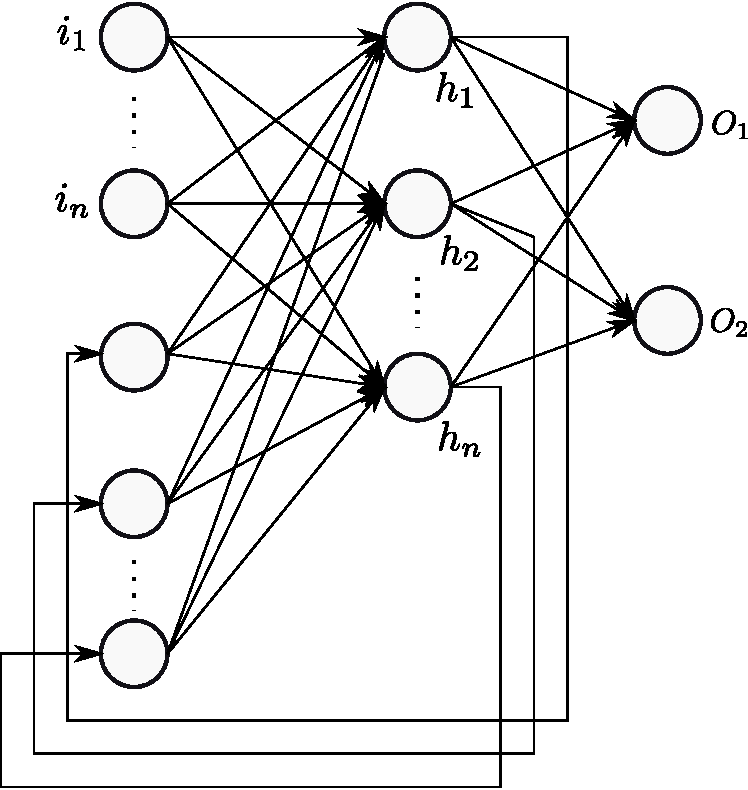
\includegraphics[width=2.6 in]{Neural_network_CF_Interaction.pdf}
    \caption{This diagram shows the structure of the classifiers used in this chapter. It is a recurrent Elman neural network~\cite{Elman1990} with $i$ input neurons, $h$ hidden neurons, and two output neurons ($O_1$ and $O_2$). $O_1$, which controls the stimulus, is fed back into the input; $O_2$ is used for making a judgment. Two bias neurons with a constant input of 1.0 are connected to each neuron of the hidden and output layers. See text for details.}
    \label{fig:neural_network_interaction}
\end{figure}

Suppose the agent responds to the level of light intensity in the environment, and we assume that the classifier could observe the agent's speed corresponding to the light intensity. One of the inputs to the classifier (network) is the light intensity in the environment at time step $t$, $I^{\left(t\right)}\in [0,1]$, and the other input is the speed $v^{\left(t\right)}$. In order to make this setup more feasible to implement, it is assumed that the system cannot directly measure the speed of the individual, but rather its position. The speed of the individual for the classifier's input is then calculated by subtracting the previous estimated position from the current estimated position, and dividing the resulting number by the time interval between two measurements.

In order to make a judgment between a model and the agent, the classifier observes the behavior (speed) over a period of time. In addition, the classifier is also in control of the light intensity in the individual's environment. At time $t=0$, the value of the light intensity is chosen randomly with a uniform distribution in the range $\left[0,1\right]$. The neural network is then updated, using $I^{\left(0\right)}$ and $v^{\left(0\right)}$. The value of the light intensity for the next time step is obtained from the classifier's output neuron $O_1$, and the process repeats. After having iterated through all the time steps (a single trial), the final value of output neuron $O_2$ is used to make a judgment: the network decides on a model if $O_2<0.5$, and on the agent if $O_2\geq0.5$. The memory (value of hidden neurons) of the classifiers is reset at the end of every trial.

\subsection{Optimization Algorithm}\label{sec:optimization_algorithm_interaction}

The algorithm used here is based on a ($\mu+\lambda$) evolution strategy with self-adaptive mutation strengths~\cite{Beyer2002, Eiben2003}. It is the same as the one used in  Chapter~\ref{ch:swarm_simulation}. For the details of the implementation, see Section~\ref{sec:optimization_algorithm_swarm}.

\subsection{Fitness Calculation}\label{sec:fitness_calculation_interaction}

Suppose the population sizes for the model and classifier are $M$ and $C$, respectively. The fitness of each model is obtained by evaluating it with each of the classifiers in the competing population ($C$ in total). For every classifier that wrongly judges the model as being the agent, the model's fitness increases by $\frac{1}{C}$. The final fitness is in $[0,1]$.

The fitness of each classifier is obtained by using it to evaluate (i) each model in the competing population ($M$ in total) once, and (ii) the agent $L$ times with different initial light intensities. For each correct judgment of the model and the agent, the classifier's fitness increases by $\frac{1}{2 \cdot M}$ and $\frac{1}{2 \cdot L}$, respectively. The final fitness is in $[0,1]$.

%The memory of the agent is never `reset' throughout the coevolutionary run---neither within the $100$ trials conducted by a single classifier, nor from one classifier to the next. (Note that this is different to our previous implementation~\citep{Li-etal2013:proc_gecco}, where the memory of the agent was `reset' after every single trial.) This makes the approach more feasible to implement as discussed in Section~\ref{sec:reducing_experiments}.

\section{Case Study One}\label{sec:case_study_one_deterministic_interaction}

The behaviors to be identified in this chapter were chosen to serve as a tractable test-bed for proof-of-concept study. While it may loosely correspond to how some animals react to the stimuli in their environment, it is not intended to mimic any specific animal. In these behaviors, non-trivial interaction with the agent is critical for leading the agent to reveal all of its behavioral repertoire. 

\subsection{Deterministic Behavior}\label{sec:deterministic_behavior_interaction}

We simulate a one-dimensional environment in continuous space. The simulation advances in discrete time steps $t \in\left\{0,1,2,\dots\right\}$. The (ambient) light intensity in the environment, $I$, can be varied continuously between $0$ and $1$. The agent distinguishes between three levels of light intensity, low ($0 \leq I < I_L$), medium ($I_L \leq I \leq I_H$), and high ($I_H < I \leq 1$). Hereafter, these levels will be referred to as $L$, $M$, and $H$.
%\footnote{In principle, the system will still work in higher dimension. As the main focus is to show how a machine interacts with the agent, for the sake of simplicity, we chose an one-dimensional environment.}

If the light intensity is at level $M$ at time $t$, the speed of the agent, $s^{\left(t\right)}\in\mathbb{R}$, varies linearly with $I^{\left(t\right)}$ as: 
\begin{equation}\label{eq:agent_behavior_linear_response}
s^{\left(t\right)}=k\left(I^{\left(t\right)}-0.5\right),
\end{equation}
where $k$ is a constant.

\begin{figure}[!t]
    \centering
    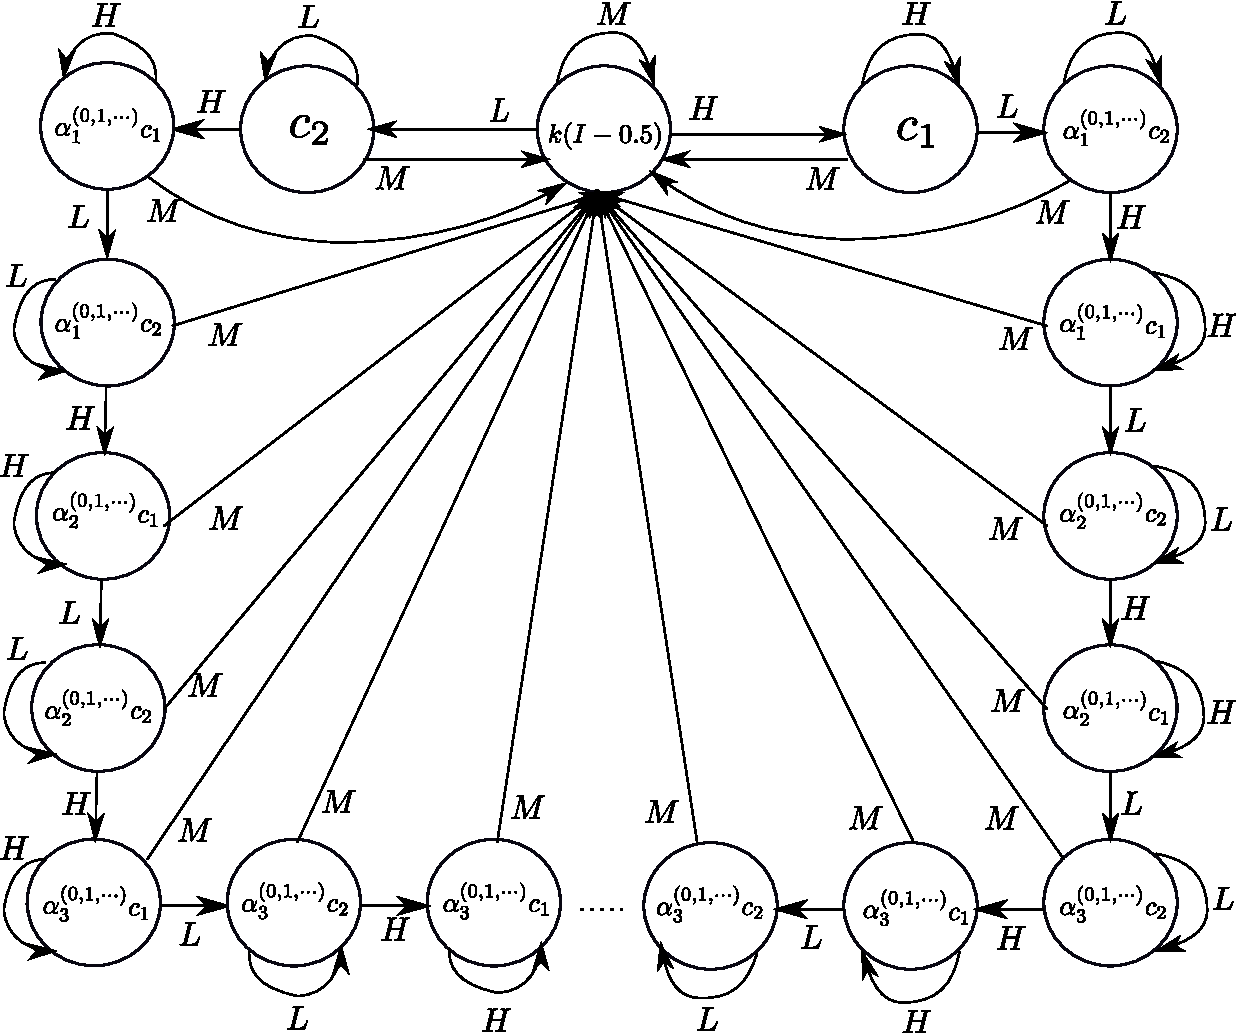
\includegraphics[width=3.5 in]{agent_behavior_deterministic.pdf}
    \caption{The deterministic behavior under investigation. It shows how the agent responses to the level of light intensity ($L$, $M$ and $H$) in its environment. Each state represents the agent's speed. See text for details.}
    \label{fig:agent_behavior_deterministic}
\end{figure}

\begin{table}[!t]
	\caption{\label{tab:example_sequence}This table shows the change of the agent's speed (shown in Figure~\ref{fig:agent_behavior_deterministic}), for an example sequence of light levels.}
	\renewcommand{\arraystretch}{1.5}
	\centering
%		\vspace{5 mm}
		\begin{tabular}{cccccccccccccc}
			\hline 
			\textbf{level} & $M$ & $H$ & $L$ & $H$ & $L$ & $L$ & $L$ & $H$ & $H$ & $L$ & $L$\tabularnewline
			\textbf{speed} & $k(I - 0.5)$ & $c_1$ & $c_2$ & $c_1$ & $c_2$ & $\alpha_{1}^{1}  c_2$ & $\alpha_{1}^{2}  c_2$ & $c_1$ & $\alpha_{1}^{1}  c_1$ & $c_2$ & $\alpha_{2}^{1}  c_2$ 					\tabularnewline  %end the row of a table
			\hline 
		\end{tabular}\\
		\vspace{5 mm}
		\begin{tabular}{ccccccccccccc}
			\hline 
			$L$ & $H$ & $H$ & $L$ & $L$ & $H$ & $H$ & $H$ & $M$ & $H$ & $L$ & $L$\tabularnewline
			$\alpha_{2}^{2}  c_2$ & $c_1$ & $\alpha_{2}^{1}  c_1$ & $c_2$ & $\alpha_{3}^{1}  c_2$ & $c_1$  & $\alpha_{3}^{1}  c_1$ & $\alpha_{3}^{2}  c_1$ & $k(I-0.5)$ & $c_1$ & $c_2$ & $\alpha_{1}^{1} c_2$\tabularnewline
			\hline 
		\end{tabular}
\end{table}

We define two constants: $c_1 = k\left(I_H - 0.5\right)$ and $c_2 = k\left(I_L - 0.5\right)$. The deterministic behavior under investigation is shown in Figure~\ref{fig:agent_behavior_deterministic}. The agent's behaviors for levels $L$ and $H$ depend on the previous levels of light intensity (i.e. the agent has memory). The two behaviors are symmetrical to each other. Here, we will describe the behavior for level $L$; the behavior for level $H$ is obtained by exchanging $L$ with $H$ and $I_L$ with $I_H$ in the following description. 

When the light intensity is at level $L$, the agent's default speed is $k\left(I_L - 0.5\right)$ and remains at that value as long as the light intensity remains at level $L$. If the light intensity is at level $H$ (for any number of time steps), and then immediately changes to level $L$, and remains at that level for at least one more time step, then the agent's speed decays exponentially with a rate of $\alpha_1$: that is, in the first time step that the light intensity is at level $L$, the agent's speed is $\alpha_1^{0}k\left(I_L-0.5\right)$; it then changes to $\alpha_1^{1} k \left(I_L-0.5\right)$, $\alpha_1^{2} k \left(I_L-0.5\right)$, and so on as long as the light intensity remains at level $L$. The agent now registers that $\alpha_1$ has been activated. If another $H\rightarrow L\rightarrow L$ sequence is observed, the agent's speed now decays exponentially with a rate of $\alpha_2$. If further $H\rightarrow L\rightarrow L$ sequences are observed, the exponential decay rate becomes and remains at $\alpha_3$. Note that at any time, if the agent observes a light intensity at level $M$, its speed is proportional to the light intensity, as shown in Eq.~\ref{eq:agent_behavior_linear_response}, and it forgets all its past observations of the light intensity (i.e., the memory of the agent is reset). 

%If the light intensity remains at level $L$ (for at least 2 consecutive time steps) immediately after changing from $H$ to $L$, the speed of the agent decays exponentially with a rate of $\alpha_1$. The agent then remembers to have `activated' $\alpha_1$; hence, in the first time step that the light intensity is at level $L$, the agent speed is $k\left(I_L-0.5\right)$; then it changes to ${\alpha_1} k \left(I_L-0.5\right)$, $\alpha_1^{2} k \left(I_L-0.5\right)$, and so on.  

%the behavior in state $H$ is obtained by replacing ``$L$'' with ``$H$'', and ``$I_L$'' with ``$I_H$'' everywhere in the following paragraph.
%If the agent immediately enters into level $L$ after level $M$, then its speed is $k\left(I_L-0.5\right)$, which is a constant, for each time step that it remains in level $L$. If one $H$/$L$ transition occurs, then the speed of the agent decays exponentially with a rate $\alpha_1$ for every time that the agent remains in level $L$. Hence, in the first time step that the agent is in level $L$, the speed is $k\left(I_L-0.5\right)$; then it changes to ${\alpha_1} k \left(I_L-0.5\right)$, $\alpha_1^{2} k \left(I_L-0.5\right)$, and so on (i.e. to observe the effect of $\alpha_1$, at least two $L$ levels occur immediately after an $H$ level). Once the effect of $\alpha_1$ has been observed, if two $H$/$L$ transitions had occurred since it has last been in level $M$, then the rate is $\alpha_2$; if three or more transitions had occurred, then the rate is $\alpha_3$. Note that the effect of $\alpha_{i+1}$ can only be observed if $\alpha_{i}$ has been observed.

The behavior of the agent can thus be represented by five cases; one where the agent's response to the light intensity is \textit{proportional} (which occurs whenever the light intensity is at level $M$); one where the agent's response is \textit{constant} (i.e. the agent's speed reaches the lower and upper saturation values ($c_1$ or $c_2$) as shown in Figure~\ref{fig:agent_behavior_deterministic}); and three where the agent's response \textit{decays exponentially} with the decay rates $\alpha_1$, $\alpha_2$ and $\alpha_3$, respectively.

Table~\ref{tab:example_sequence} shows an example sequence of light levels, along with the corresponding speed of the agent (i.e., the speed shown in Figure~\ref{fig:agent_behavior_deterministic}). 

Here, $I_L$ and $I_H$ are set to $0.1$ and $0.9$ respectively.  $k$ is set to $1.25$; hence, the lower and the upper saturation values of the speed are $k\left(I_L - 0.5\right) = -0.5$ and $k\left(I_H - 0.5\right) = 0.5$. The exponential decay rates are set to: $\alpha_1=0.8$, $\alpha_2=0.4$, $\alpha_3=0.2$. Thus, in each case, the agent's speed decays exponentially towards zero. Note that these values ($k$, $\alpha_1$, $\alpha_2$ and $\alpha_3$) are chosen arbitrarily and the coevolutionary algorithm is not sensitive to them. 
%The value of $I_L$/$I_H$ are chosen to be a small/large number in $[0,1]$, so that it is relatively hard to randomly generate a sequence of high and low level of light intensity.

The system identification task is to learn these four parameters ($k$, $\alpha_1$, $\alpha_2$ and $\alpha_3$) of the agent. It is worth while to mention again that to learn $\alpha_3$, the machine needs to at least output the sequence: $H\rightarrow L\rightarrow L\rightarrow H\rightarrow L\rightarrow L\rightarrow H\rightarrow L\rightarrow L$ or $L\rightarrow H\rightarrow H\rightarrow L\rightarrow H\rightarrow H\rightarrow L\rightarrow H\rightarrow H$. Since $I_L$ and $I_H$ are set to a relatively small and large value in $[0,1]$ respectively, it is very unlikely to randomly generate such sequences.

\subsection{Simulation Setup}\label{sec:simulation_setup_deterministic_interaction}

We use three setups for the \textit{Turing Learning} method. The setup, in which the classifier is in control of the light intensity in the agent's environment, is hereafter referred to as the ``Interactive'' setup. In order to validate the advantages of the interactive approach, we compared it against the situation where the classifier only observes the agent in a passive manner; that is, it does not control the light intensity in the environment. We considered two such setups: in the first setup (hereafter, ``Passive 1'') the light intensity is randomly chosen from the uniform distribution in $\left[0,1\right]$, in every time step. In the second setup (hereafter, ``Passive 2''), the light intensity is randomly chosen only after certain number of time steps (in this setup the number is chosen to be 10). All other aspects of these two setups are identical to the ``Interactive'' setup. 

The population sizes of the models and classifiers are chosen to be $100$, respectively. We performed $100$ coevolution runs for each setup. Each coevolution run lasts $1000$ generation. In one generation, each classifier conducts $100$ trials on the agent. In each trial, the classifier observes the agent for $\unit[10]{s}$ at $\unit[0.1]{s}$ intervals, that is, a total of $100$ data points.

\subsection{Results}\label{sec:results_interaction_deterministic}

\begin{figure}[!t]%
	\centering
	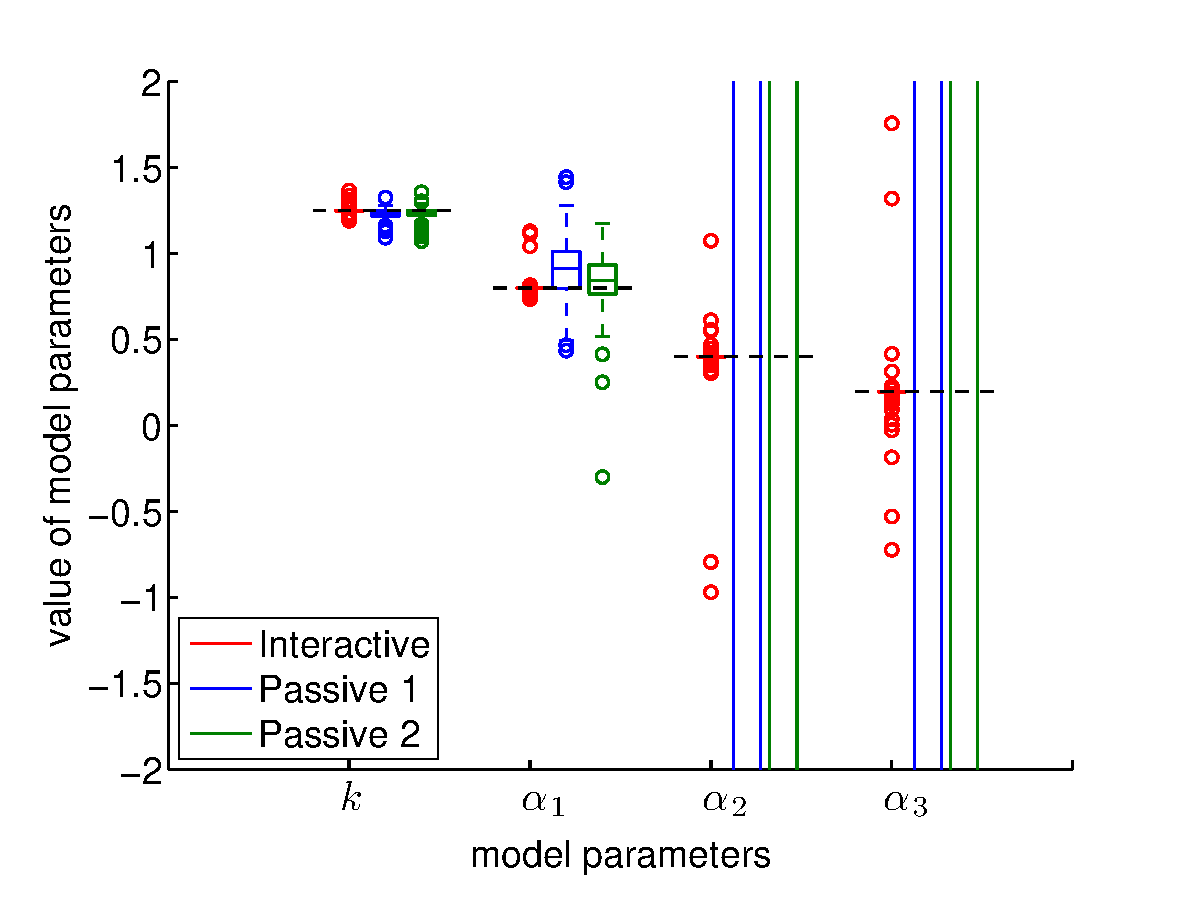
\includegraphics[width=3 in]{parameters_compare_without_noise}
	\caption{This plot shows the distributions of the evolved models with the highest subjective fitness in the $1000^\textrm{th}$ generation in the coevolutions. Each box corresponds to $100$ coevolution runs. The dotted lines correspond to the values of the four parameters that the system is expected to learn (i.e. those of the agent). From top to bottom, these are 1.25, 0.8, 0.4, 0.2, respectively. Note that in order to zoom in on the relevant range, some boxes and outliers are omitted from the plot.\label{fig:parameters_compare_without_noise}}
\end{figure}

\subsubsection{Analysis of Evolved Models}\label{sec:analysis_evolved_models_deterministic_interaction}

Figure~\ref{fig:parameters_compare_without_noise} shows a box plot with the distributions of the evolved models with the highest subjective fitness in the $1000^\textrm{th}$ generation over $100$ coevolution runs of the three setups. The passive coevolutions are able to evolve the parameters $k$ and $\alpha_1$ with a reasonable accuracy; however, they are not able to evolve $\alpha_2$ and $\alpha_3$. In the Passive 1 coevolution, the relative errors of the medians of the four evolved parameters ($k,\alpha_1,\alpha_2,\alpha_3$) with respect to those of the agent are $1.2\%$, $14.3\%$, $7.8\times10^4\%$, and $2.3\times10^5\%$, respectively. The Passive 2 coevolution leads to similarly large relative errors in the evolved values of $\alpha_2$ and $\alpha_3$. This phenomenon can be explained as follows. If the light intensity changes randomly (either every time step, or every ten time steps), it is unlikely that the 
$H\rightarrow L\rightarrow L$ and/or $L\rightarrow H\rightarrow H$ sequences 
%transitions $L$ to $H$ and/or $H$ to $L$ 
will occur enough times, without a level of $M$ in between, such that the classifiers can observe the effects of $\alpha_2$ and $\alpha_3$. Therefore, the classifiers do not evolve the ability to distinguish the behavior of models from the behavior of the agent with respect to these two parameters, and in turn, these parameters do not converge to their true value in the model population.

In contrast to the passive coevolutions, the Interactive coevolution is able to evolve all the four parameters with a good accuracy. The relative median errors are $0.024\%$, $0\%$, $0.025\%$ and $0.15\%$ for $k$, $\alpha_1$, $\alpha_2$ and $\alpha_3$ respectively. This implies that by the $1000^{\textrm{th}}$ generation, the classifiers have learned how to control the pattern of the light intensity in such a way that they can distinguish models from the agent based on the effect of any of the four parameters. Therefore, in order to compete for being selected in the population, the models are evolved to behave like the agent in every aspect.

\begin{figure}[!t]%
	    \centering
		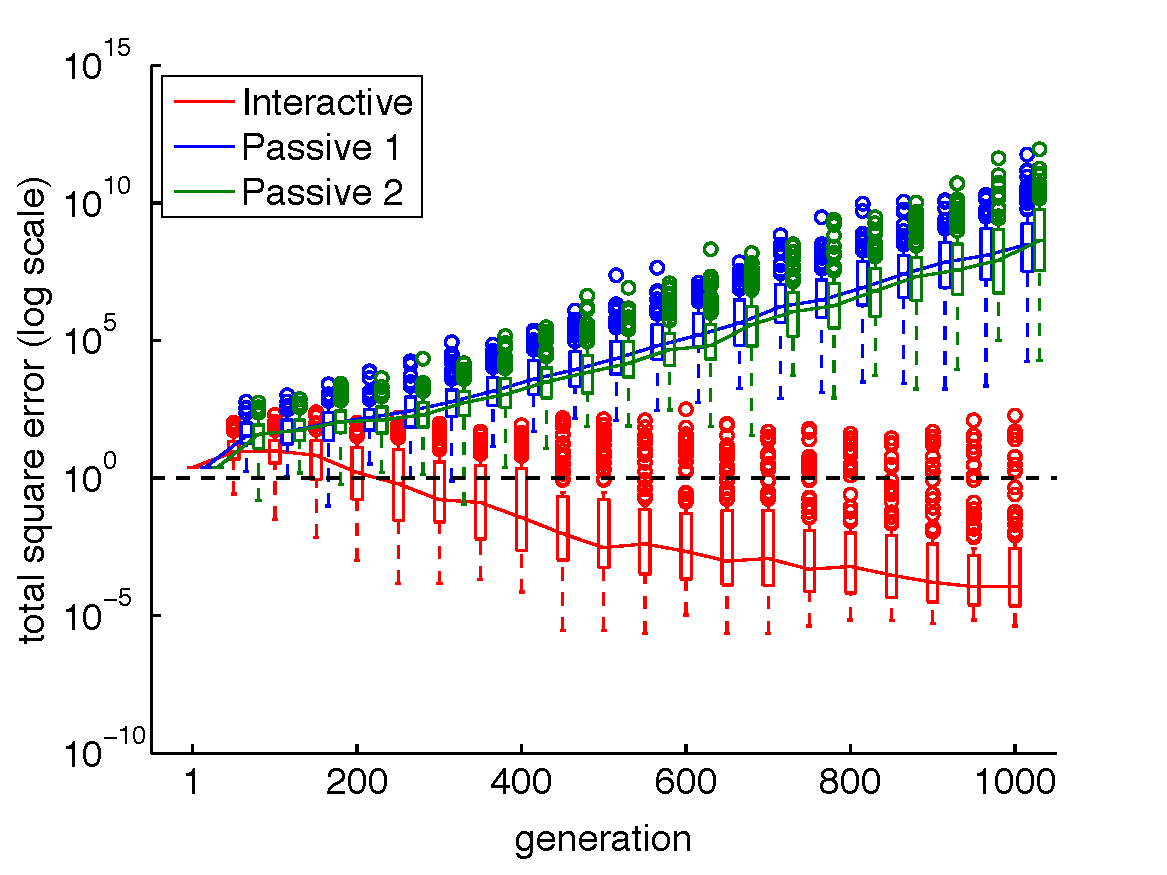
\includegraphics[width=3 in]{convergence_compare_without_noise}
		\caption{This plot shows the total square errors of the evolved model parameters compared to those of the agent over generations. The models with the highest subjective fitness in each generation are selected. Each box corresponds to $100$ coevolution runs, and the solid lines correspond to the median error.\label{fig:convergence_compare}}
\end{figure}

\begin{figure}[!t]%
	   \centering
	   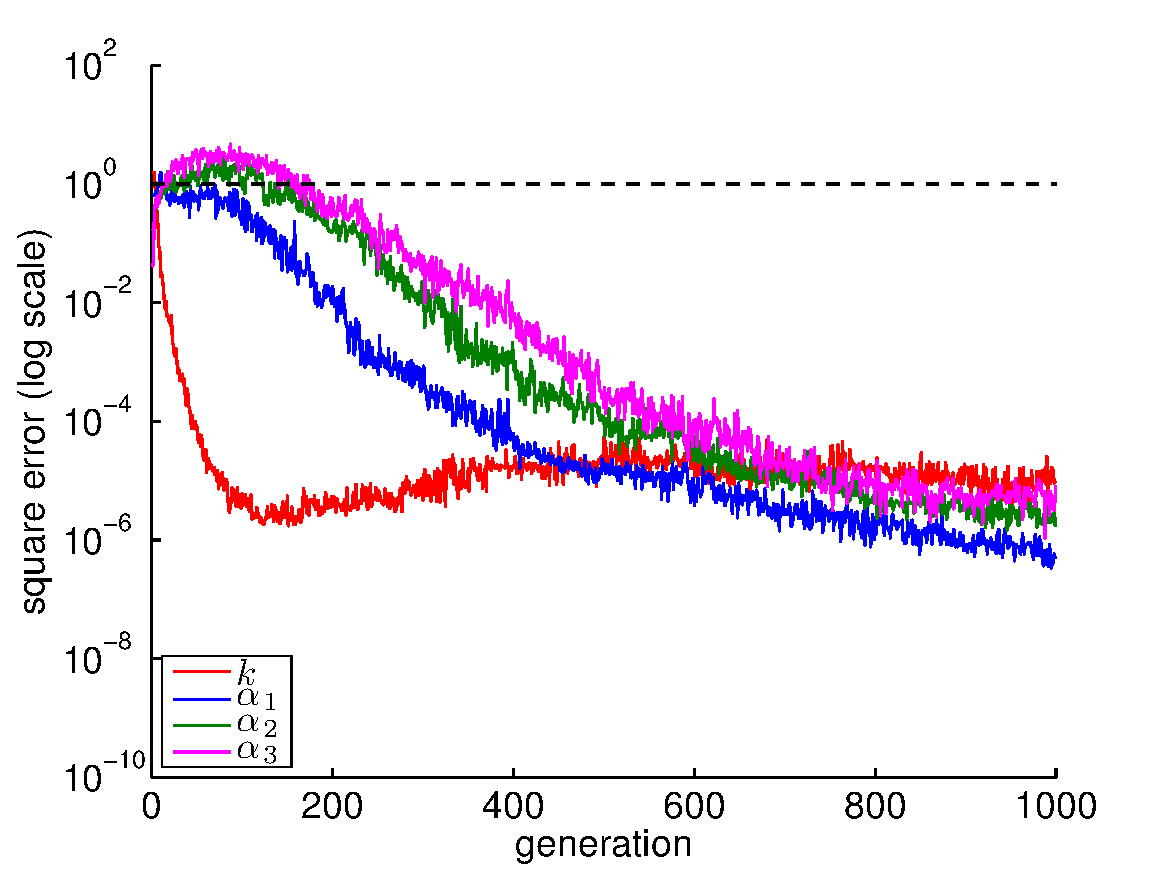
\includegraphics[width=3 in]{parameters_convergence_without_noise}
	    \caption{This plot shows how the square error in the individual model parameters
	    changes over the generations in the Interactive coevolution. The curves correspond to median values from $100$ coevolution runs.\label{fig:parameters_convergence}}
\end{figure}

\begin{figure}[!t]%
	\centering
		\subfloat[Interactive coevolution \label{fig:fitness_without_noise_auto}]{%
			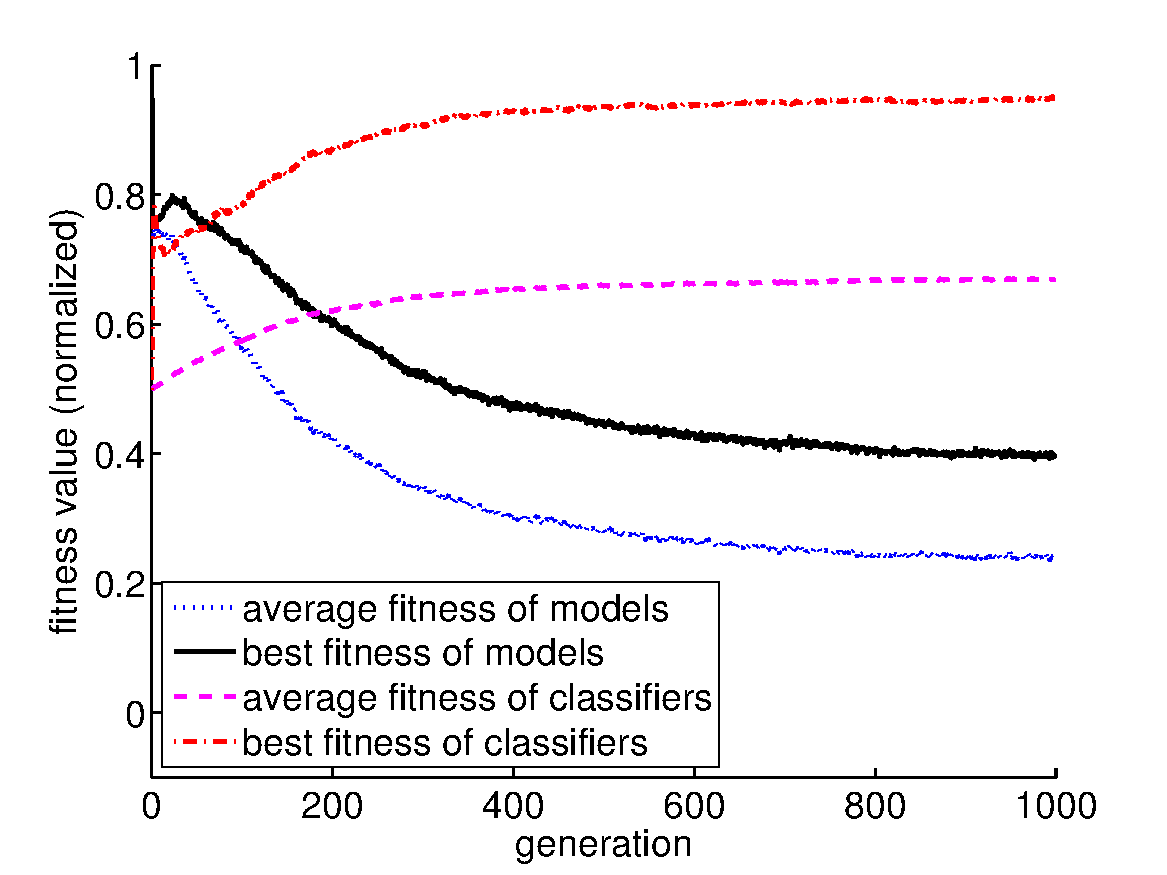
\includegraphics[width=3 in]{fitness_without_noise_auto}
		}\\
		\subfloat[Passive 1 coevolution \label{fig:fitness_with_noise_random_1}]{%
			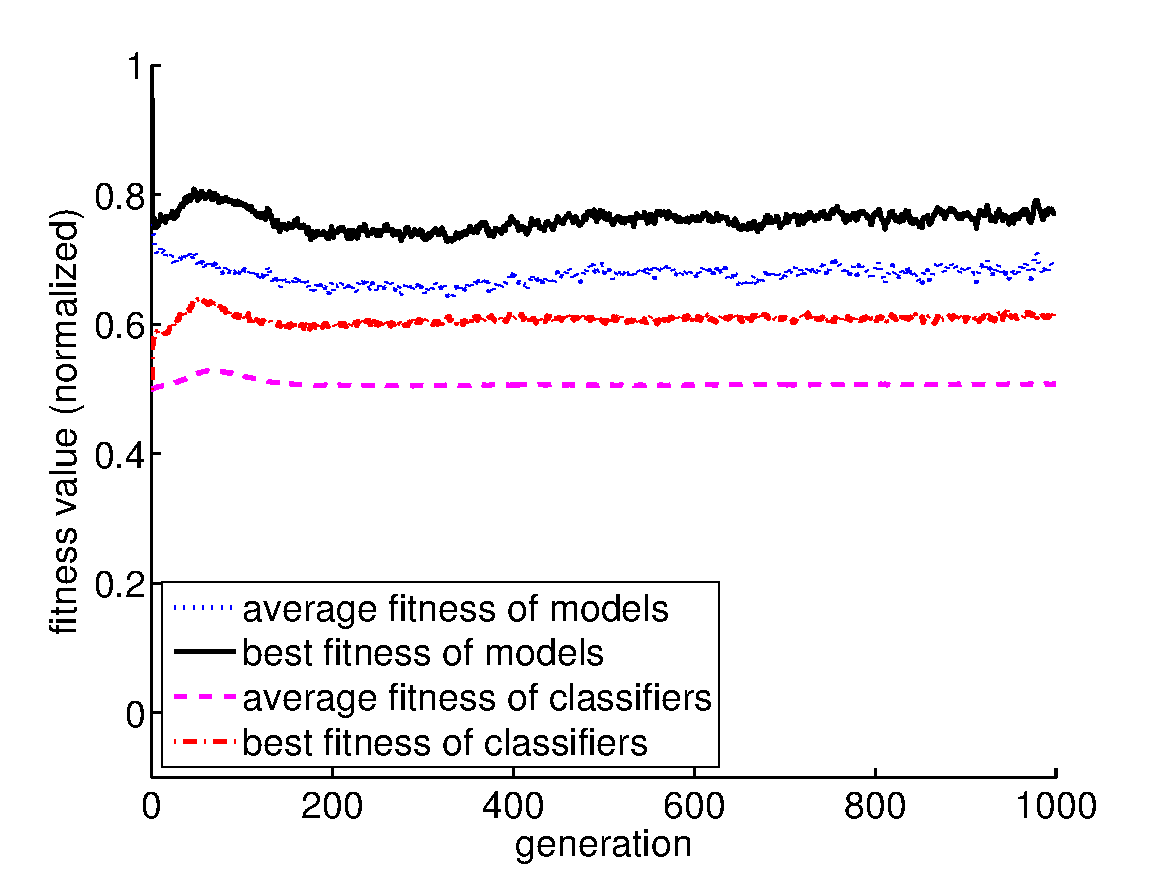
\includegraphics[width=3 in]{fitness_without_noise_random_1}
		}\\
		\caption{This plot shows the subjective fitness (normalized) of the classifiers and
		the models in (a) the Interactive coevolution, and (b) the Passive 1 coevolution.
		The curves show the average fitness across $100$ coevolution runs.\label{fig:fitness_dynamics}}
\end{figure}

\subsubsection{Coevolutionary Dynamics}\label{sec:coevolutionary_dynamic_deterministic_interaction}

Figure~\ref{fig:convergence_compare} shows the dynamics of the coevolutionary algorithms. The horizontal axis shows the generation, whereas the vertical axis shows the total square error of the model parameters, that is, the sum of the square errors in the four parameters (of the model with the highest subjective fitness in each generation) with respect to their true values. In the case of the Interactive coevolution, the median error starts to reduce after around the $100^\textrm{th}$ generation,  and keeps decreasing until the last generation where it reaches a value of $10^{-4}$. In contrast, in the case of the passive coevolutions, not only does the median error not decrease, but it increases to a value of $10^{8}$ by the $1000^\textrm{th}$ generation.

We now analyze how the four individual parameters evolve during the course of the Interactive coevolution, which is the only fully-successful setup. The plot shown in Figure~\ref{fig:parameters_convergence} reveals how the learning proceeds in the coevolution. Parameter $k$ is the first to be learnt, followed by $\alpha_1$, while parameters $\alpha_2$ and $\alpha_3$ take a longer time to approximate the true values. This means that the classifiers first learn to distinguish models from the agent on the basis of $k$ and $\alpha_1$. This ability of the classifiers drives the model population to evolve $k$ and $\alpha_1$, in order to mislead the classifiers. Eventually, the classifiers also learn to exploit the effects of $\alpha_2$ and $\alpha_3$ in order to make the right judgment; thereby driving the model population to evolve these two parameters accurately. After about the $600^\textrm{th}$ generation, the learning of the four parameters proceeds with approximately identical rates.

In order to analyze why the Interactive coevolution is successful while the passive ones are not, we can look at the dynamics of the subjective fitnesses of the classifiers and the models (as defined in Section~\ref{sec:fitness_calculation_interaction}) during the course of the coevolution. As both of the passive coevolutions fail to converge, we present the analysis of fitness dynamics only for Passive 1 coevolution (the other case was found to have similar dynamics). Figure~\ref{fig:fitness_dynamics} shows the fitness dynamics of the Interactive and the Passive 1 coevolutions. In the case of the Interactive coevolution (see Figure~\subref*{fig:fitness_without_noise_auto}), the average fitness of the classifiers starts off at $0.5$, which means that the classifiers make judgments that are no better than random judgments. However, the classifiers quickly improve in fitness, which in turn causes the fitness of the models to decrease. This increases the selective pressure on the models. After about $600$ generations both the fitness of classifiers and models reach a steady state, which according to Figure~\ref{fig:parameters_convergence} corresponds to the region where the four parameters evolve with virtually identical rates. In the case of the Passive 1 coevolution (see Figure~\subref*{fig:fitness_with_noise_random_1}), the average fitness of the classifiers also starts off at $0.5$. In the first few generations, this increases slightly, because the classifiers learn how to distinguish models from the agent on the basis of parameters $k$ and $\alpha_1$. However, the models quickly adapt to this new ability of the classifiers. Now, as the classifiers are unlikely to have the opportunity to observe the effects of $\alpha_2$ and $\alpha_3$, their average fitness returns to $0.5$. This leads to a disengagement phenomenon, in which there is no more meaningful selection in the model population, therefore leading the parameters $\alpha_2$ and $\alpha_3$ to drift, the effect of which can be seen in Figure~\ref{fig:convergence_compare}.

\subsubsection{Analysis of Evolved Classifiers}\label{sec: analysis_evolved_classifiers_deterministic_interaction}

In this section, we analyze the evolved classifiers in the Interactive coevolution. The model described in Section~\ref{sec:model_deterministic_interaction} is defined by four parameters: $\{ k, \alpha_1, \alpha_2,\alpha_3 \}$. In order to evaluate the quality of the evolved classifiers we performed a grid search over the space of the amount of disturbance (i.e. noise) injected into each of the four parameters. We used 11 noise magnitude settings per parameter, $M\in\{0, 0.1, \dots, 1\}$, with the noise being added to the parameters as follows:
\begin{equation}\label{eq:noise_on_magnitudes}
p^{\prime} = p(1 + \mathcal{U}(-M, M)),
\end{equation}
where $p\in\{ k, \alpha_1, \alpha_2,\alpha_3 \}$ represents any of the four parameters, and $\mathcal{U}(-M,M)$ denotes a uniform distribution on the interval $(-M,M)$. Note that $M=0$ corresponds to no noise, whereas $M=1$ means that the noisy value of the parameter can be between $0$ and twice its actual value.

%Manhattan distance
\begin{figure}[!t]
	\centering
			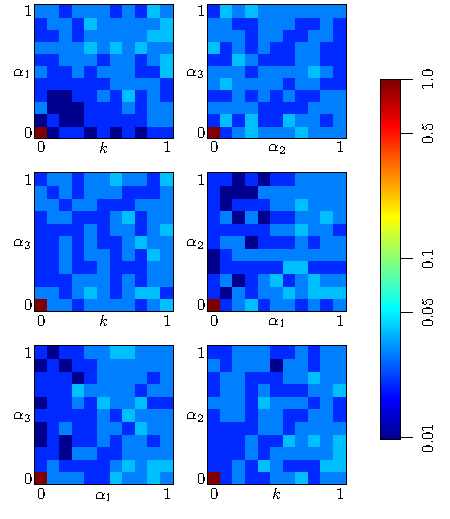
\includegraphics[width=3 in]{grid_visualization_random.pdf}
		\caption{This figure shows the landscape of $U^{*}$ (log scale) for the overall best classifier over the six sub-spaces with two parameters as degrees of freedom (from $100$ coevolution runs). Each axis in each plot ranges between 0 and 1, corresponding to the minimum and maximum magnitude of noise added into each parameter respectively. See text for details.\label{fig:grid_search}}
\end{figure}

\begin{figure}[!t]
		\centering
		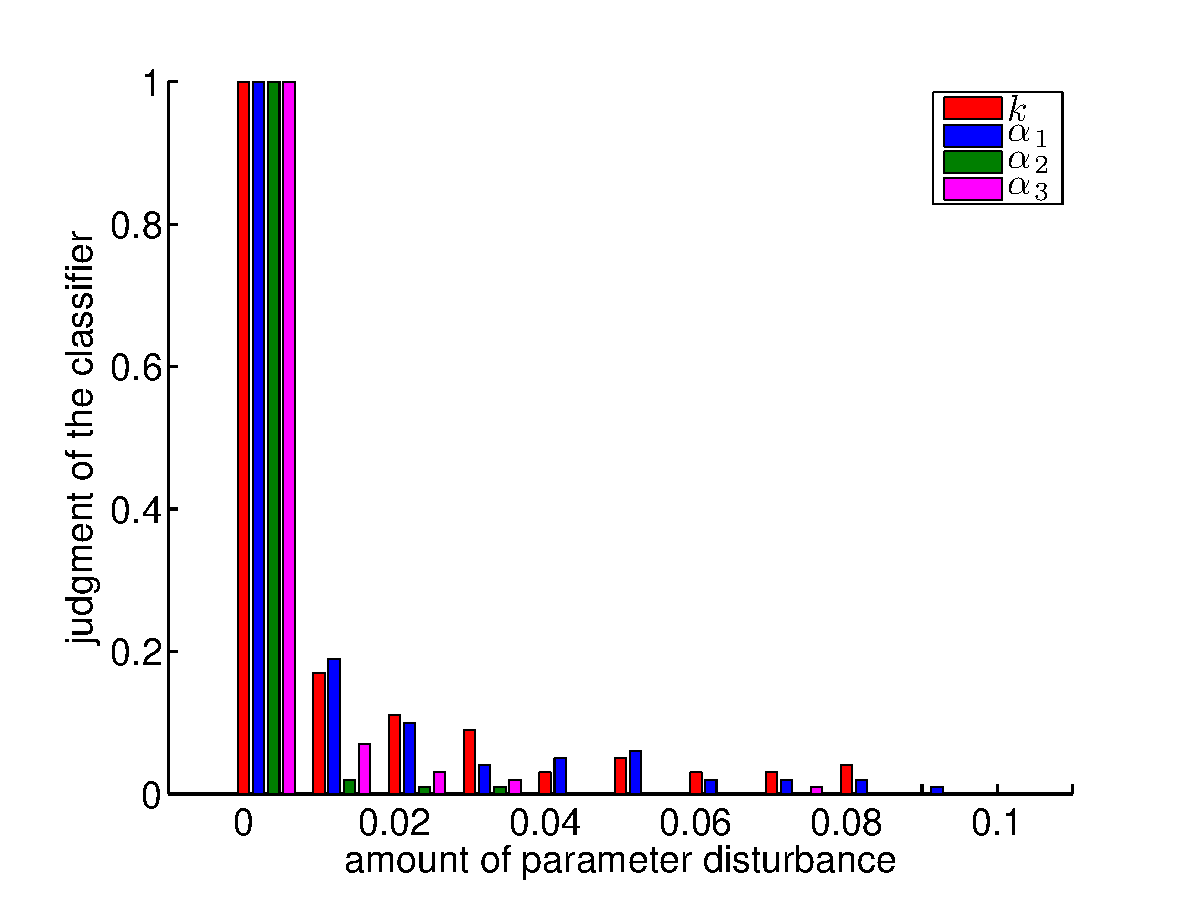
\includegraphics[width=3 in]{classifier_accuracy_higher_resolution}
		\caption{This plot shows the average judgment [$U$, see Eq.~\ref{eq:performance_metric_model}] of the best evolved classifier over 100 trials when the magnitude of noise added into each parameter of the agent is within 0.1.\label{fig:classifier_accuracy_higher_resolution}}
\end{figure}

\begin{figure*}[!t]
	\centering
			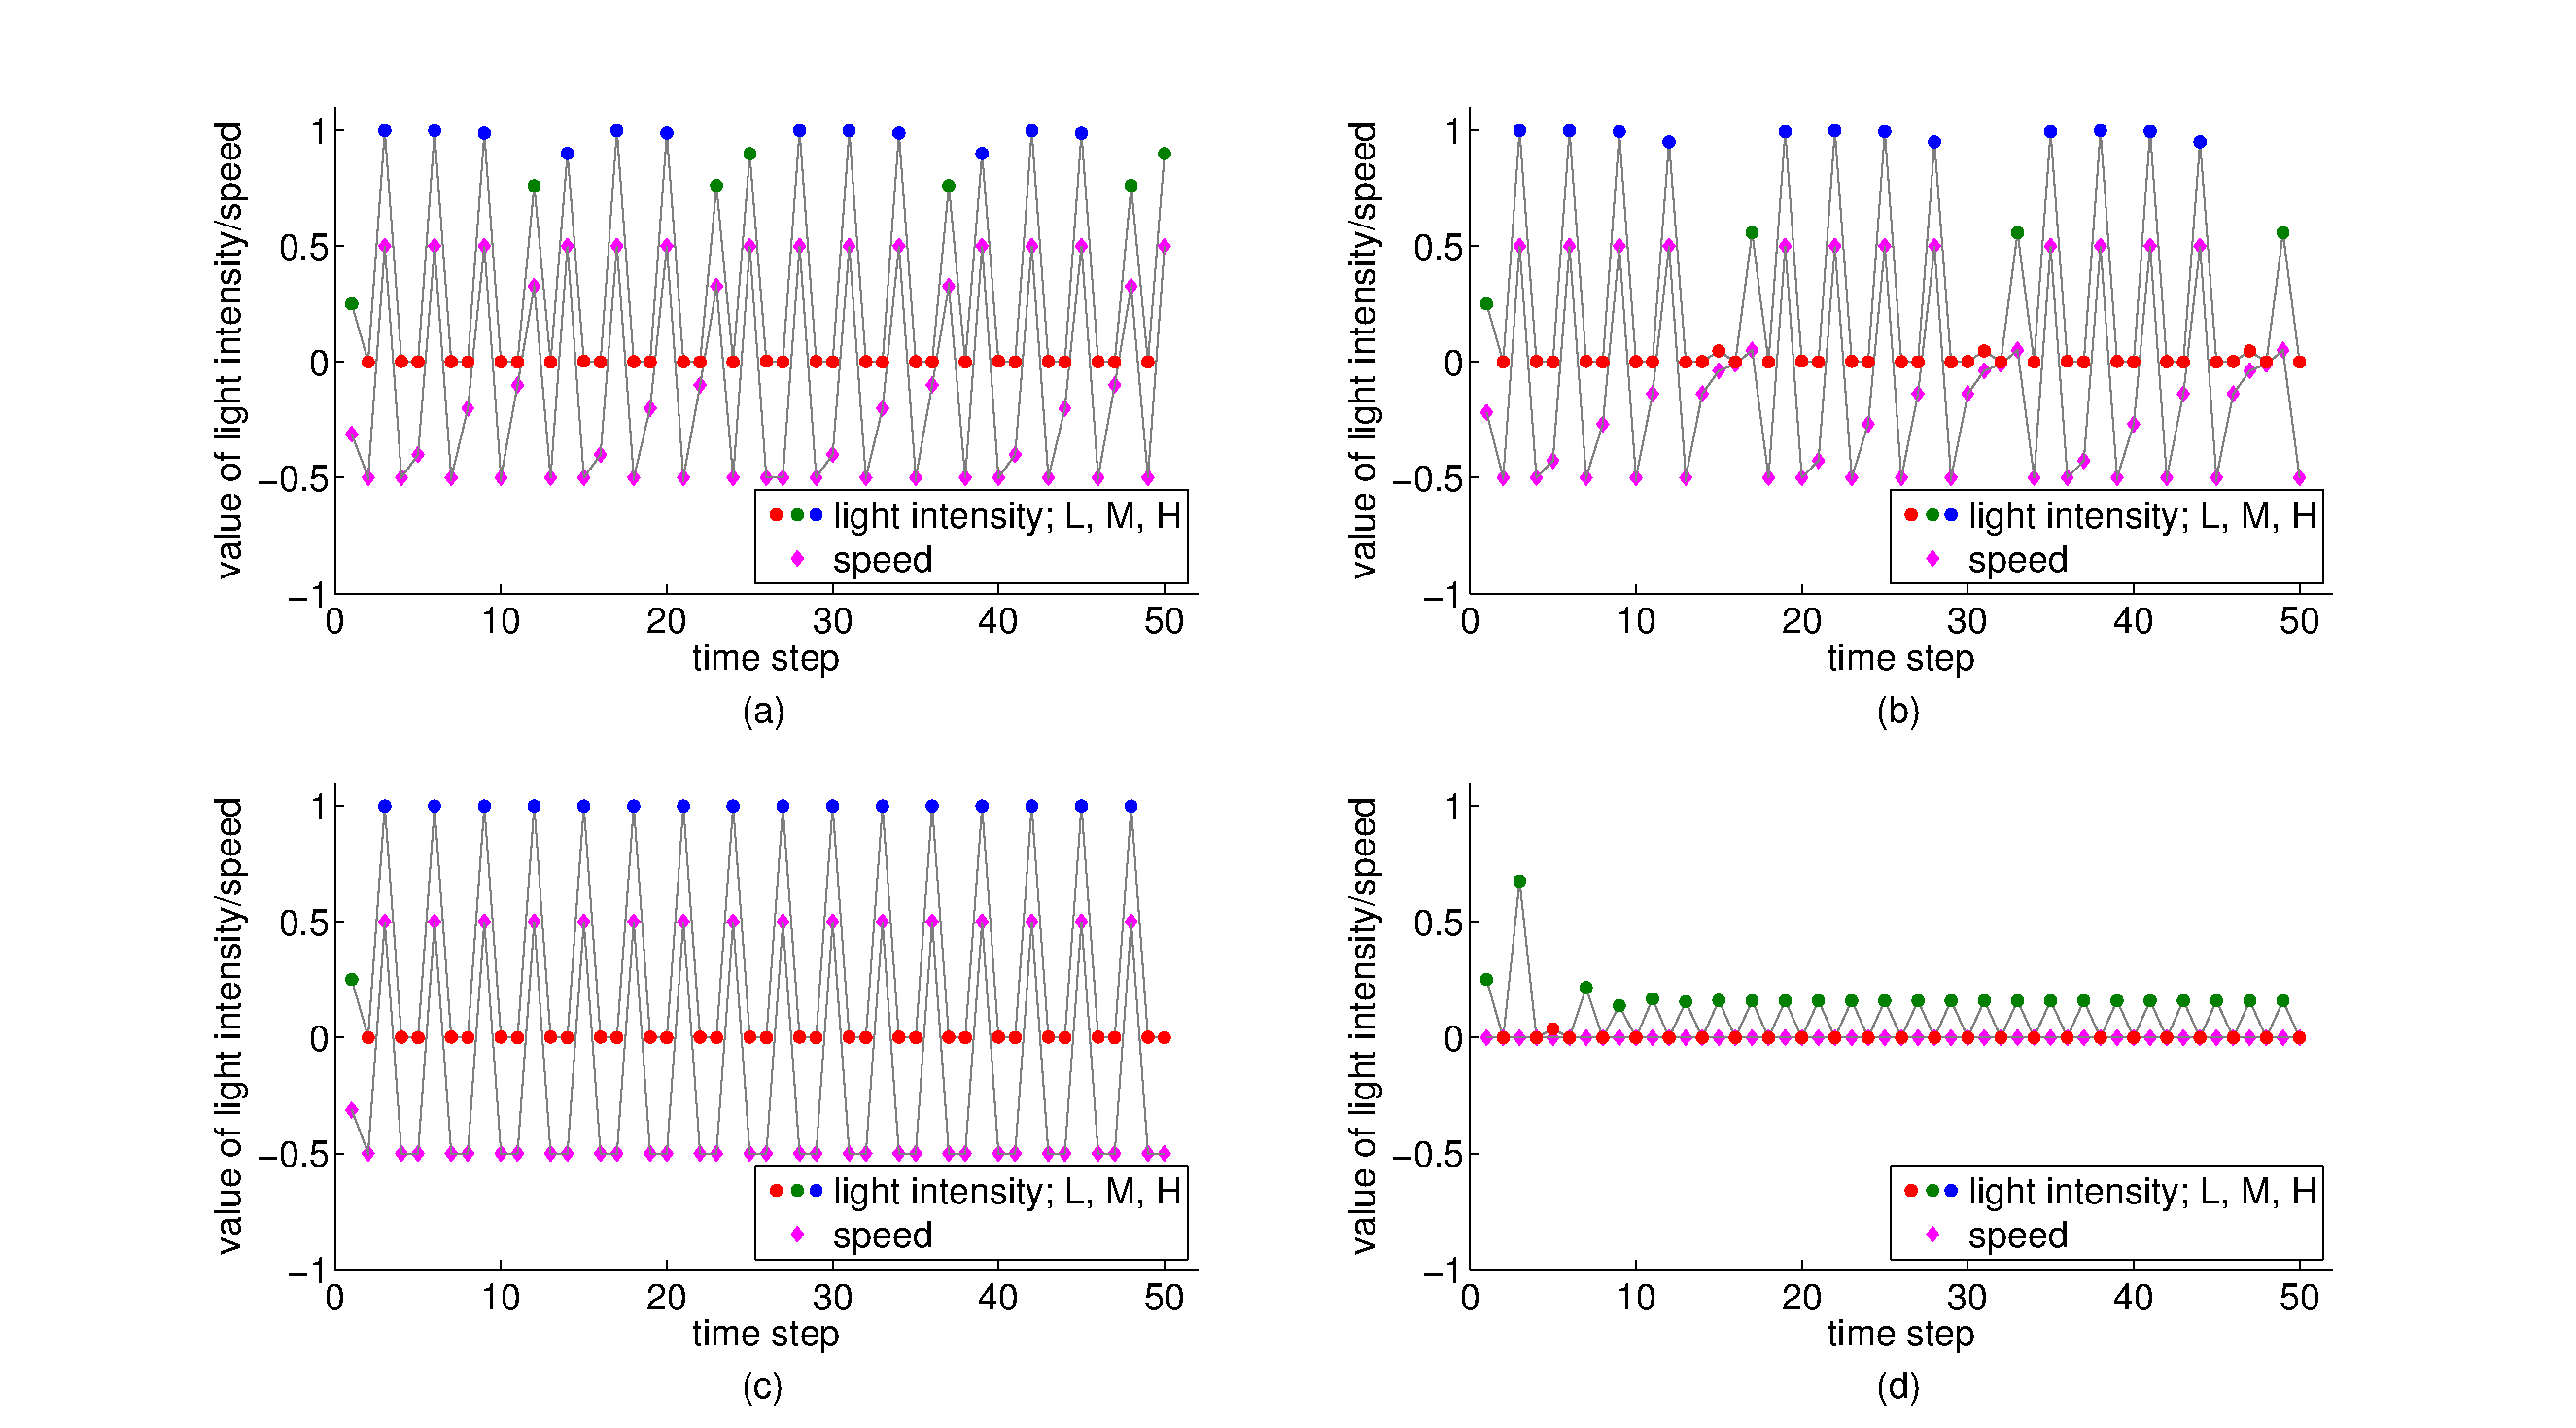
\includegraphics[width=6.0 in, height = 3.5in]{light_intensity_output}
			\caption{This plot shows the light intensity sequences as output by the overall best classifier (circular points), along with the corresponding speeds of the agents (diamond-shaped points) in four trials conducted on different agents: (a) the agent; (b) a model similar to the agent, generated randomly according to Eq.~\ref{eq:noise_on_magnitudes} with $M=0.5$; (c) a model whose speed is linear to the light intensity; and (d) a static model, whose speed is always $0$ (i.e. $k=0$).
The colors of the circular points (red, green, blue) correspond to light intensities at levels $L$, $M$ and $H$, respectively.\label{fig:post_evaluation_light_output}}
%		\caption{This plot shows the sequences of light intensity (circle) in the environment as controlled by the best evolved classifier as well as the corresponding speeds (diamond) of the agent/models in independent four trials with the same initial light intensity. The three different colors (red, blue, green) of the circle correspond to the three levels of light intensity, which are $H$, $M$ and $L$ respectively. These four trials are conducted independently on the four different agents respectively: (a) the agent; (b) the randomly generated model; (c) the static model (i.e. its speed is always 0, regardless of the change of light intensity); (d) the model without exponential decay (i.e. its speed only follows the basic curve in  Figure~\ref{fig:agent_behavior}). See the text for detail.\label{fig:post_evaluation_light_output}}
\end{figure*}

For the sake of simplicity, we only analyzed the classifiers with the highest subjective fitness in the last generation of the 100 coevolutions. For each of the 100 classifiers, and for each combination of noise magnitudes, we conducted 100 trials. In other words, we conducted $100 \cdot 11^4 \cdot 100 = 146,410,000$ trials in total. 
% (normally no need to repeat this)
%In each trial, the light intensity at time zero was initialized randomly with a uniform distribution over the interval $(0, 1)$.
In each trial, we modulated the agent's parameters according to Eq.~\ref{eq:noise_on_magnitudes}.
% (not relevant, as no different from before)
Each trial was run for T = 100 time steps (the same setting used within the coevolutions). 
For each combination of magnitudes employed, the overall performance $U$ was computed as the sum of the final judgments of the classifier in each trial, divided by the total number of trials, $N$: 
\begin{equation}{\label{eq:performance_metric_model}}
U = \sum\limits_{i = 1}^{N} {{J_i}}/N,
\end{equation}
where, $J_i\in\{0,1\}$ is the final judgment of the classifier in trial $i$, and $N$ is the total number of trials conducted. Note that $J_i = 0$ and $J_i = 1$ imply that the classifier has judged the behavior as being that of a model and the agent, respectively.

In order to find the overall best classifier from the 100 classifiers analyzed, we defined the following metric:  

%\begin{equation}{\label{eq:performance_metric_classifier}}
%\begin{split}
%W &= \frac{1}{W_\textrm{max}} \sum \limits_{i = 1}^{6} \Bigg[ \frac{1} {({U_i}^{*} \left(0, 0\right)+1)} \quad + \\ & \quad \sum \limits_{\begin{smallmatrix} j, k %%%\in \lbrace 0, 0.1, \dots, 1.0 \rbrace ^2, \\ j^2+k^2 \neq 0 \end{smallmatrix}} \left( M_{j}+M_{k} \right) {U_i}^{*} \left(j, k\right) \Bigg], 
%\end{split}
%\end{equation}

\begin{equation}
\begin{split}
W &= \left[1 - U\left(0,0,0,0\right)\right] \\
& + \frac{1}{\Omega} \mathop{\sum \sum \sum \sum}_{\begin{smallmatrix} i, j, k, \ell \in \lbrace 0, 0.1, \dots, 1 \rbrace \\ i^2 + j^2+k^2 + \ell^2 \neq 0 \end{smallmatrix}} \left(i+j+k+\ell\right) U\left(i,j,k,\ell\right),
\end{split}
\label{eq:performance_metric_classifier}
\end{equation}
where $\Omega=29282$ is the maximum value that the quadruple sum can achieve (i.e. if all the $U$'s are equal to $1$). The first term in Eq.~\ref{eq:performance_metric_classifier} penalizes the classifier if $U<1$ when there is no noise on the parameters; they are thus undisturbed and identical to the ones of the agent. The second term penalizes the classifier if $U>0$ for any non-zero noise combination, with increasing penalties being applied to higher noise magnitudes. The normalization of the second term by $\Omega$ serves to make the two terms contribute equally to $W$, which can take values in $[0,2]$. Note that the minimum value of $W=0$ can only be achieved by the perfect classifier, that is, one that outputs 1 if $i=j=k=\ell=0$ and $0$ otherwise. In our case, the best classifier achieved a value of $W=3.7\cdot 10^{-3}$.

%where, $W_{\textrm{max}}$ which is equivalent to $36.25$, is the maximum value of $W$ that a classifier can get. The first term in the square bracket corresponds to the reciprocal of the average of the classifier' s judgments (see Eq.\ref{eq:performance_metric_model}) when the parameters are noise-free. The second term corresponds to the sum of the average of the classifier' s judgments weighted by the sum of two noise magnitudes. When the agent is subjected to noise, this metric punishes large value of $W$, but gives increasing rewards to a classifier that has small values of $W$ for larger noise magnitudes. Furthermore, it penalizes small values of $W$ when the parameters are noise-free. The best overall classifier is the one that obtains the smallest value of $W$.

The performance landscape of the models is $5$-dimensional ($4$ model parameters plus performance measure), and cannot be visualized directly. Therefore, we considered each combination of two model parameters ($\binom{4}{2}=6$ combinations) as a sub-space, and for each point in this sub-space, we calculated the performance measure as the maximum value over the sub-space spanned by the remaining two parameters. For instance, on the sub-space $\left(k, \alpha_1\right)$, the performance measure $U^{*}\left(k, \alpha_1\right)$ was calculated as:
\begin{equation}
U^{*}\left(k, \alpha_1\right) = \max_{\alpha_2,\alpha_3} 
U\left(k, \alpha_1, \alpha_2, \alpha_3\right).
\label{eq:max_operation}
\end{equation}
Note that for all the points except $(0,0,0,0)$, Eq.~\ref{eq:max_operation} corresponds to the worst-case scenario for the classifiers, because the value of $U$ for the ideal classifier at these points is $0$. For the point $(0,0,0,0)$, the value of $U$ for the ideal classifier is $1$. 

Figure~\ref{fig:grid_search} shows the landscape of $U^{*}$ (log scale) for the overall best classifier over the six sub-spaces.
% From the data of the grid search, we have found that t
When interacting with the agent (i.e. $i=j=k=\ell=0$), the output of the classifier is always 1. This corresponds to the point $U^{*}(0,0)$ in the six sub-spaces of Figure~\ref{fig:grid_search} (here only the maximum is shown). When interacting with the models (i.e. when the parameters of the agent are perturbed), for any combination of noise magnitudes, the average output of the classifier is
%The output is close to 0, if the parameters of the agent are perturbed. When the magnitude of the noise is 0.1 or above, the maximum output of the classifier is very low---
below 0.05 for the six sub-spaces. 
%This means the classifier is able to categorize the model correctly, if its parameters are different from those of the agent. 
%Also, we can see that the classifier is very sensitive to the disturbance of each parameter. When the magnitude of the noise is 0.1 or above, the maximum output of the classifier is very low---below 0.05 for all 6 sub-spaces. This means the classifier can always distinguish between the agent and the models. 
%From the data of grid search, we have found that on each of the 6 sub-spaces shown in Figure~\ref{fig:grid_search}, the value shown at 

In order to further analyze how sensitive the overall best classifier is when the parameters of the agent are only slightly perturbed, we set the maximum magnitude of noise added to each parameter to 0.1, and used a resolution of 0.01. In this evaluation, we only injected noise into one parameter at a time. For each noise magnitude, the classifier was evaluated in 100 trials (with different initial light intensities, and randomly-generated noise), and the average performance measure was computed according to Eq.~\ref{eq:performance_metric_model}. 

Figure~\ref{fig:classifier_accuracy_higher_resolution} shows the average judgment [$U$, see Eq.~\ref{eq:performance_metric_model}] of the best classifier, which was evaluated in 100 trials. With increasing noise magnitudes, the average judgment of the classifier approaches zero, which means that the classifier can identify the agents as models more consistently. The classifier has different sensitivities to the four parameters; the effects of noise on $\alpha_2$ and $\alpha_3$ on its judgment are higher than those of $k$ and $\alpha_1$. For instance, in the case of $\alpha_2$, even with $M=0.01$, the classifier correctly judges the behavior as being that of a model in 98\% of the trials. As we have seen, $k$ and $\alpha_1$ are the first two parameters to be identified in the coevolution. $\alpha_2$ and $\alpha_3$ are addressed in the later generations of the coevolutionary process, and it seems that the classifier is more sensitive to these two parameters.
%Therefore, the classifier needs to identify $\alpha_2$ and $\alpha_3$ in the later generations of coevolutionary process, and consequently, it learns to output more light intensity points that alternate between $H$ and $L$ (as can be seen in Figure~\ref{fig:post_evaluation_light_output_repeat}). This leads it to specialize to $\alpha_2$ and $\alpha_3$, explaining why by the 1000$^\textrm{th}$, it is most sensitive to these two parameters.

We now investigate how the overall best classifier interacts with the agents. We conducted four trials with four different agents: (a) the agent; (b) a model similar to the agent, generated randomly according to Eq.~\ref{eq:noise_on_magnitudes} with $M=0.5$; (c) a model whose speed is linear to the light intensity without exponential decay (i.e. $k=1.25$, $\alpha_1 = \alpha_2 = \alpha_3 = 1$); and (d) a static model, whose speed is always $0$ (i.e. $k=0$). In each trial, the initial light intensity was set to $0.25$. The trials lasted for $100$ time steps. 

Figure~\ref{fig:post_evaluation_light_output} shows the sequences of light intensity output by the classifier, along with the speed of the agents in the four trials, for the first $50$ time steps (we observed that the last $50$ time steps constitute a repetition of the first $50$).
%Figure~\ref{fig:post_evaluation_light_output} shows, over 50 time steps, the sequences of light intensity chosen by the classifier as well as the corresponding speeds of the agent/models in independent four trials with the same initial light intensity. Each trial lasts 100 time steps (as used within the coevolution); however, the plot only shows the sequences of light intensity for the first 50 time steps, as  those for the other 50 time steps are repetitive. Here, the initial value of light intensity was chosen to be 0.5, which means the agent/models were static and their memory was cleared at the beginning of the trial. However, it is worth mention that the classifier produces the same light intensity sequence, irrespective of the initial light intensity. These four trials were conducted on the four different agents respectively: (a) the agent. (b) the randomly generated model; in this case, the model was randomly generated with some disturbance on each parameter of the agent according to Eq.~\ref{eq:noise_on_magnitudes}. The magnitude of the noise added into each parameter was chosen to be 0.5. (c) the static model. That is, the model does not move no matter how the light intensity changes. (d) the model without exponential decay, which means the speed of this model only follows the basic curve in  Figure~\ref{fig:agent_behavior}, and the exponential decay rate is 1.
%We now investigate how the overall best classifier interacts with the agent and the models. Figure~\ref{fig:post_evaluation_light_output} shows, over 50 time steps, the sequences of light intensity chosen by the classifier as well as the corresponding speeds of the agent/models in independent four trials with the same initial light intensity. Each trial lasts 100 time steps (as used within the coevolution); however, the plot only shows the sequences of light intensity for the first 50 time steps, as  those for the other 50 time steps are repetitive. Here, the initial value of light intensity was chosen to be 0.5, which means the agent/models were static and their memory was cleared at the beginning of the trial. However, it is worth mention that the classifier produces the same light intensity sequence, irrespective of the initial light intensity. These four trials were conducted on the four different agents respectively: (a) the agent. (b) the randomly generated model; in this case, the model was randomly generated with some disturbance on each parameter of the agent according to Eq.~\ref{eq:noise_on_magnitudes}. The magnitude of the noise added into each parameter was chosen to be 0.5. (c) the static model. That is, the model does not move no matter how the light intensity changes. (d) the model without exponential decay, which means the speed of this model only follows the basic curve in  Figure~\ref{fig:agent_behavior}, and the exponential decay rate is 1.
As we can see, the classifier outputs different sequences of light intensity in order to interact with the different agents. The greater the difference between a model and the agent, the more varied is the sequence of light intensities that the classifier outputs when interacting with it as compared to the one it outputs when interacting with the agent. For the agent, the classifier repeatedly outputs a $H\rightarrow L\rightarrow L$ sequence, in order to fully reveal the behavior (this is analyzed in detail in the following paragraph). For the model that is similar to the agent (see Figure~\ref{fig:post_evaluation_light_output}\textcolor{blue}{(b)}), the sequence of light intensities is similar to the one produced for the agent, but it is not identical. Interestingly, for the model without exponential decay (see Figure~\ref{fig:post_evaluation_light_output}\textcolor{blue}{(c)}), the classifier produces the $H\rightarrow L\rightarrow L$ sequence even more often than it does for the agent, but it does not set the light intensity to level M. For the static model (see Figure~\ref{fig:post_evaluation_light_output}\textcolor{blue}{(d)}), the classifier never outputs a $H\rightarrow L\rightarrow L$ sequence; instead, it outputs a sequence that alternates between $M$ and $L$.
%For example, in Figure~\ref{fig:post_evaluation_light_output}a, the classifier keeps outputting $H\rightarrow L\rightarrow L$ sequence in order to reveal the full behavior of the agent (which is analyzed in detail in the following paragraph). However, when the model is static, the classifier never outputs such sequence. Instead, it only outputs a sequence between $M$ and $L$. Interestingly, when the model does not decay exponentially, the classifier keep producing $H\rightarrow L\rightarrow L$ sequence even more often than it does for the agent. It seems that the classifier wishes to `explore' the \textit{exponential decay} behavior of this model. For the randomly generated model, the sequence of light intensity is more similar to that for the agent, as the behavior of this model is close to that of the agent. 

We now focus on analyzing the behavior of the agent in Figure~\ref{fig:post_evaluation_light_output}\textcolor{blue}{(a)}. Initially, the classifier outputs the sequence $L \rightarrow H\rightarrow L\rightarrow L \rightarrow H\rightarrow L\rightarrow L\rightarrow H\rightarrow L\rightarrow L\rightarrow M$, which means that by the $12^\textrm{th}$ time step, it has already observed the effects of all four parameters. Interestingly, the classifier then (essentially) repeats this sequence and thus observes the effect of all the parameters for another seven times (four repetitions occur in the last 50 time steps, which are not shown in Figure~\ref{fig:post_evaluation_light_output}\textcolor{blue}{(a)}). We conjecture that the repetitions make the classifier more robust in determining whether the behavior under observation is that of a model or the agent.
%The classifier produces an almost identical light intensity sequence, irrespective of the initial light intensity. As the initial light intensity is the only source of randomness  (which is random). If the light intensity sequences in two agent experiments is exactly the same, the classifier will make the same judgment whenever the system is free of any noise. 
%Initially, the classifier outputs a sequence alternating between $H$ and $L$, which means that by the $12^\textrm{th}$ time step, it has already observed the effects of all four parameters. Interestingly, the classifier then repeats this process and observes the effect of all four parameters for seven more times. We conjecture that these repetitions make the decision making more robust.
% TODO - these numbers are probably wrong now: 10 trials, 12th time step, seven more times
These results suggest that the classifier succeeds in controlling the level of ambient light in a way that helps distinguish between the agent and the models, revealing all aspects of the underlying behavior. Note that the classifiers are not provided with any prior information about the agent, including its structure. Thus, all knowledge is gained through an evolutionary process that is driven by the accuracy of their judgments.
%Note that the classifier does not have prior information about the model structure, and thus
%in order to maximize its rewards during the coevolutionary process and distinguish between the agent and the models
%even though it had no prior information about the structure they share (e.g. distinct light levels) and it is unable tond the agent or models parametis unaware of the structure they share (e.g., the distinct  is not provided with any prior information about the model structure and parameters.

\subsubsection{Noise Study}\label{sec:noise_study_deterministic_interaction}

\begin{figure}[!t]
		\centering
		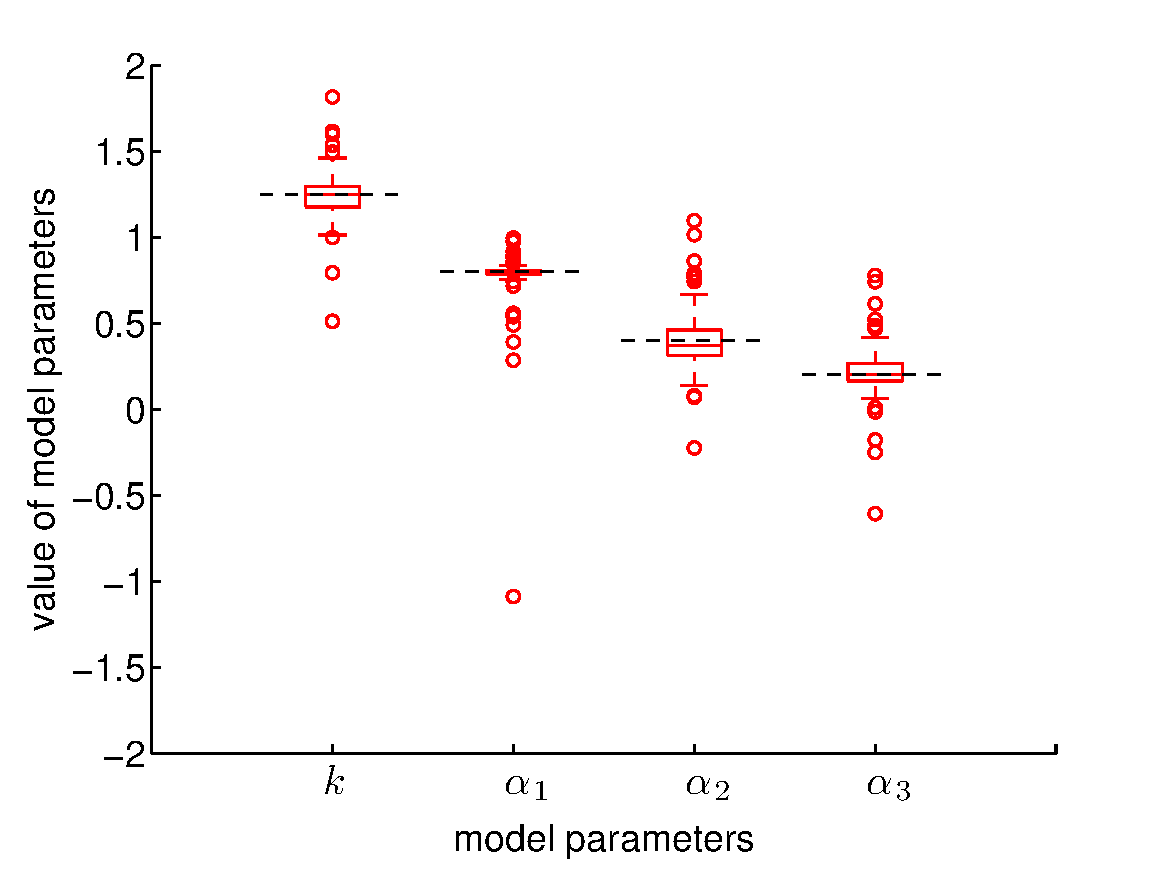
\includegraphics[width=3.2 in]{parameters_with_noise_interactive}
		\caption{This plot shows the distributions of the evolved models with the highest subjective fitness in the $1000^\textrm{th}$ generation of the Interactive coevolution with noise (for a comparison to the case without noise, see Figure~\ref{fig:parameters_compare_without_noise}). The dotted lines correspond to the values of the four parameters that the system is expected to learn (i.e. those of the agent). From top to bottom, these are 1.25, 0.8, 0.4, 0.2, respectively. \label{fig:parameters_compare_with_noise}}
\end{figure}

%\begin{figure}[!t]
%		\centering
%		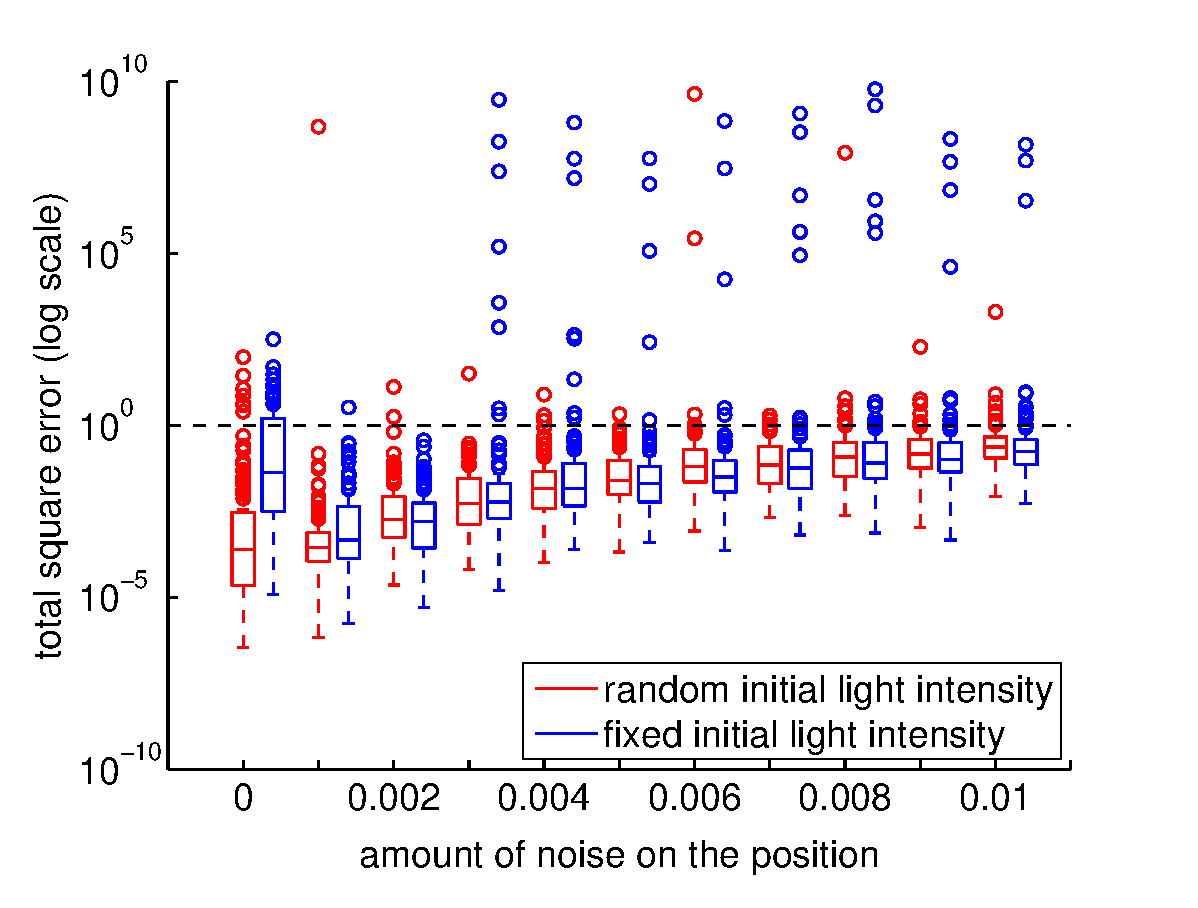
\includegraphics[width=3.2 in]{square_error_noise_random_fix_light}
%		\caption{This plot shows the total square error of the evolved models with the highest subjective fitness in the $1000^\textrm{th}$ generation with an increasing amount of noise added on the positional measurements of the agent. Each box corresponds to $100$ coevolutionary runs. Note that at a noise level of 0.01, the relative error in the estimated speed introduced by two consecutive positional measurements can be up to $40\%$, even if the agent moves at the maximum speed. See the text for more details. \label{fig:square_error_noise_random_fix_light}}
%\end{figure}
%Note that when the noise added on the position is 0.01, it corresponds to a minimum of $20\%$ noise on the agent speed.

We now consider the situation where, during the coevolutionary process, noise is injected into the agent's behavior, and the agent's positions as measured by the system. This makes the overall setup more realistic as the locomotion of agents and any tracking system will be affected by noise and measurement error. Since the passive coevolutions fail even in the noiseless case, we consider only the Interactive coevolution for the sake of simplicity. We performed $100$ coevolutionary runs with the following settings. The light intensity perceived by the agent at time $t$ is obtained by multiplying the actual intensity by a random number generated uniformly in $\left(0.95,1.05\right)$, and capping the perceived intensity to $1$ if it exceeds this value. Noise is also applied to the speed of the agent by multiplying the original speed with a random number generated uniformly in $\left(0.95,1.05\right)$. Noise on the estimated position on the agent is applied by adding a random number generated from a normal distribution: $\mathcal{N}\left(0,0.005\right)$. 

Figure~\ref{fig:parameters_compare_with_noise} shows a box plot with the distributions of the evolved models with the highest subjective fitness in the $1000^\textrm{th}$ generation of the Interactive coevolution with noise. The effect of the noise is to widen the distribution of the evolved parameters across the $100$ coevolutionary runs; however, the median values of the evolved parameters are still very close to the true values. Interestingly, the Interactive coevolution does not seem to learn $\alpha_2$ and $\alpha_3$ significantly worse than it does learn $k$ and $\alpha_1$. 
%The relative errors of the medians of the four evolved parameters are $0.19\%$, $0.15\%$, $7.0\%$ and $0.85\%$ for $k$, $\alpha_1$, $\alpha_2$ and $\alpha_3$, respectively. 

%We now wish to investigate how sensitive the system is to one particular type of noise. Here, we consider noise on the agent's position, since tracking is more likely subjected to noise when conducting physical experiments. In each time step, the position is corrupted by adding some noise following a normal distribution $\mathcal{N}(0, \sigma)$, with $\sigma\in \{0, 0.001, 0.002, \dots, 0.01\}$. The agent's absolute displacement in a single time interval, at the maximum speed is $0.5\cdot 0.1 = 0.05$. At a noise level of 0.01, the relative error in the estimated speed introduced by the two positional measurements can then be up to $40\%$. The relative error is even higher when the agent does not move at the maximum speed. We performed two sets of coevolutionary runs:
%%Note that when the magnitude of noise added on the position is 0.01, it corresponds to a minimum of $20\%$ noise on the agent speed, since the maximum speed of the agent is $0.5$ and the time interval is 0.1s. If the classifiers observe the effect of $\alpha_3$ (i.e. the agent speed is no bigger than $0.5\times0.2=0.1$), the percentage could be more than $100\%$. 
%
%\begin{itemize}
%\item \textit{Random Initial Light Intensity}: In the first set of 100 coevolutionary runs, the initial light intensity for the model/agent in each trial conducted by a classifier is chosen randomly in $[0,1]$, as done in the previous sections.
%\item \textit{Fixed Initial Light Intensity}: We conducted another 100 coevolutionary runs where the initial light intensity is fixed. The value is randomly chosen  in $[0,1]$ at the beginning of each run, and then remains constant within that run.
%\end{itemize}
%%As we discussed in Section~\ref{sec: analysis_of_the_evolved_classifiers}, the best classifier always outputs the same sequence even if the initial light intensity in each trial is generated randomly. Therefore we conducted another 100 coevolutionary runs where the initial light intensity is chosen randomly in $(0,1)$ at the start of each run, and then remain constant within that run (i.e. for every trial performed by all the classifiers).
%Figure~\ref{fig:square_error_noise_random_fix_light} shows the total square error of the evolved models with the highest subjective fitness in the $1000^\textrm{th}$ generation with increasing amounts of noise. In the case of \textit{Random Initial Light Intensity}, the total square error is not significantly different between the noiseless case and the case with the least amount of noise being injected (0.001). With an increasing amount of noise, the performance of the evolved models degrades gracefully.
%\begin{figure}[!t]%
%	\centering
%		\subfloat[without noise\label{fig:fitness_without_noise_fix_light}]{
%			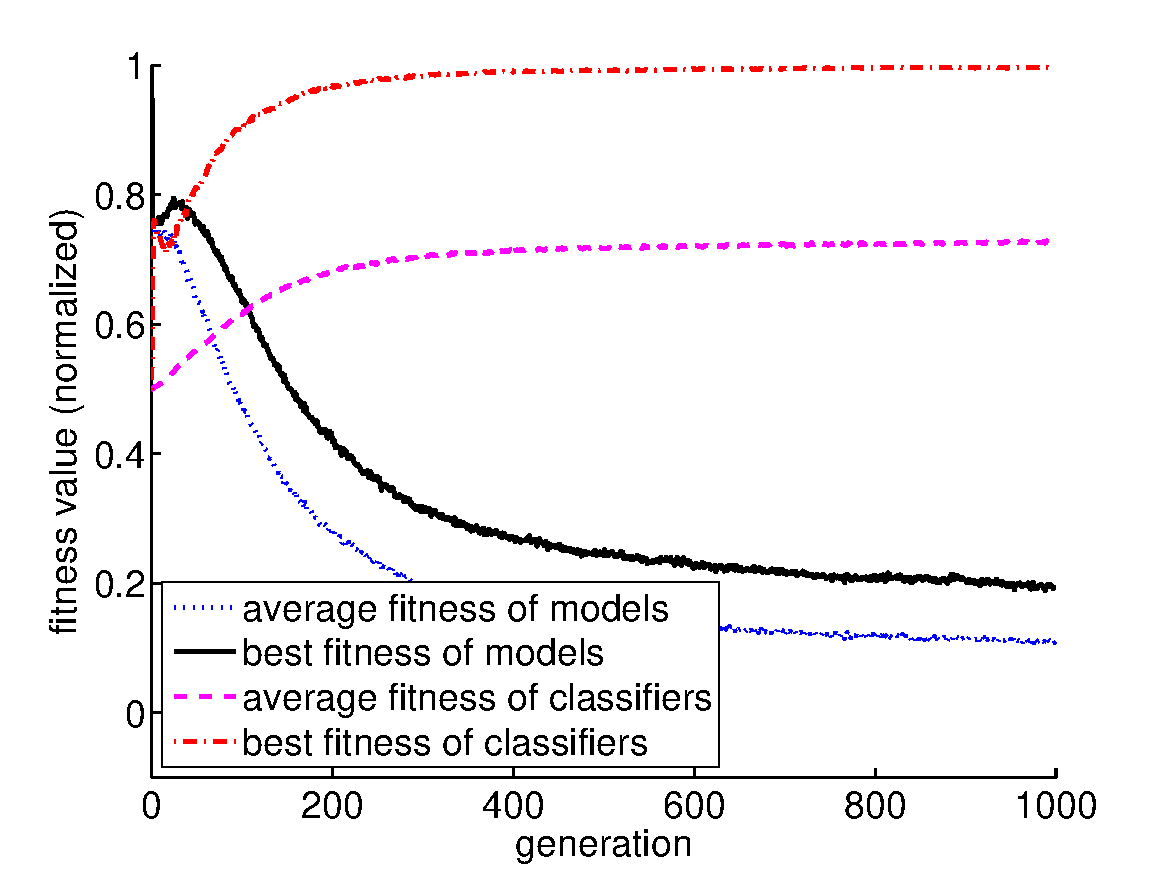
\includegraphics[width=3 in]{fitness_without_noise_fix_light}
%		}\\
%		\subfloat[with noise\label{fig:fitness_with_noise_fix_light}]{
%			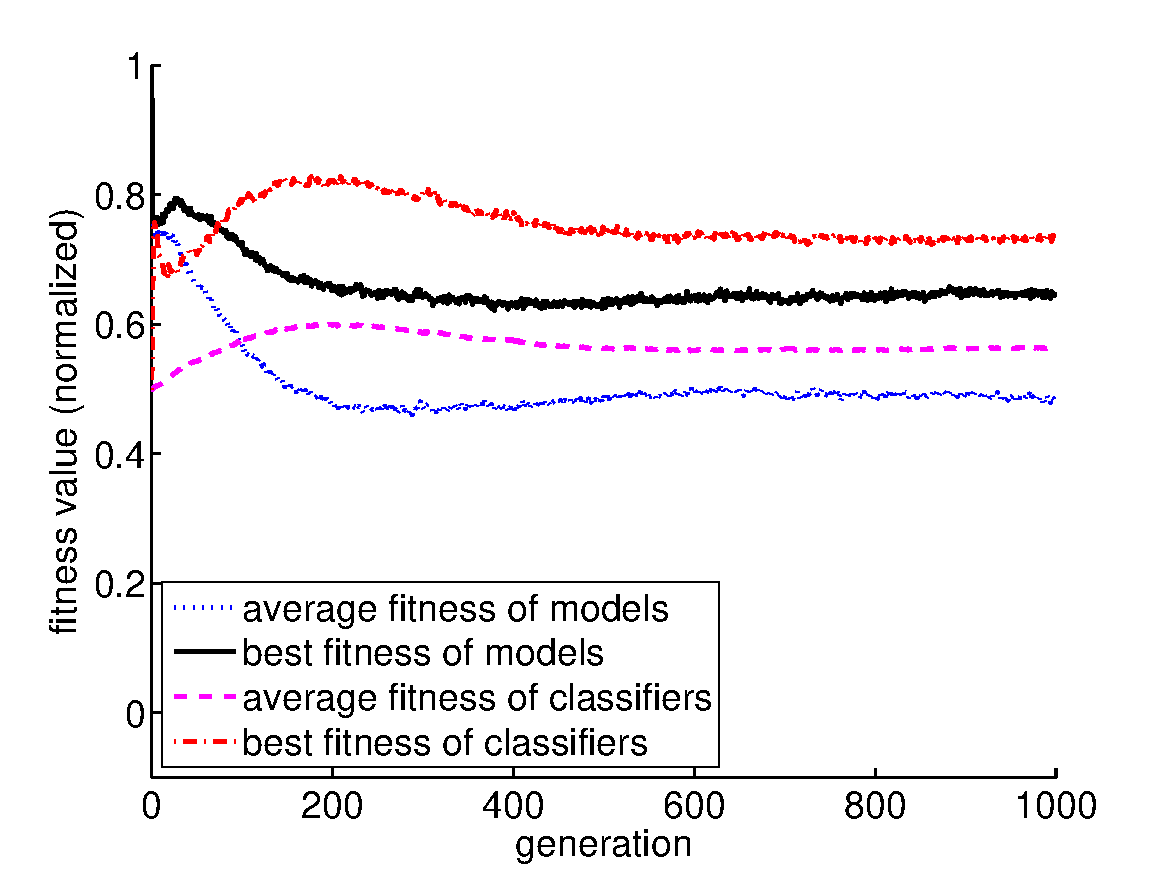
\includegraphics[width=3 in]{fitness_with_noise_fix_light}
%		}\\
%		\caption{This plot shows the subjective fitness (normalized) of the classifiers and
%		the models in the Interactive coevolution with fixed initial light intensity (a) without noise, and (b) with noise. The magnitude 
%		of noise added onto the position is 0.001. The curves show the average fitness across $100$ coevolutionary runs.
%		\label{fig:fitness_dynamics_fix_light}}
%\end{figure}
%
%In the case of \textit{Fixed Initial Light Intensity}, the system learns significantly better with a certain amount of noise ($ \leq 0.005$) than without noise (two-sided Mann-Whitney test, 5$\%$ significance level). To explain this further, we look at the dynamics of the subjective fitness of both evolved classifiers and models during the coevolutionary process, as shown in Figure~\ref{fig:fitness_dynamics_fix_light}. In Figure~\subref*{fig:fitness_without_noise_fix_light}, we can see that the fitness of the classifiers is much higher than that of the models. The average fitness of models drops to below 0.2 after about the $300^\textrm{th}$ generation, and continues to decrease thereafter. This means that the models can hardly compete with the classifiers. Moreover, the model population seems to lack diversity, as the average and the best fitnesses of the models are relatively close to each other. When some noise is injected into the system, the fitness of the models and the classifiers remains ``balanced'' (see Figure~\subref*{fig:fitness_with_noise_fix_light}). The gap between the best and the average fitnesses of the models is almost twice as much as that in the case of no noise. This means that moderate noise help maintain the diversity of the coevolutionary process, which leads to a better accuracy of the evolved models compared with the case without noise.

\subsubsection{Using a Single-Population Evolutionary Algorithm}\label{sec:single_population_EA_deterministic_interaction}
\begin{figure}[!t]
	\centering
	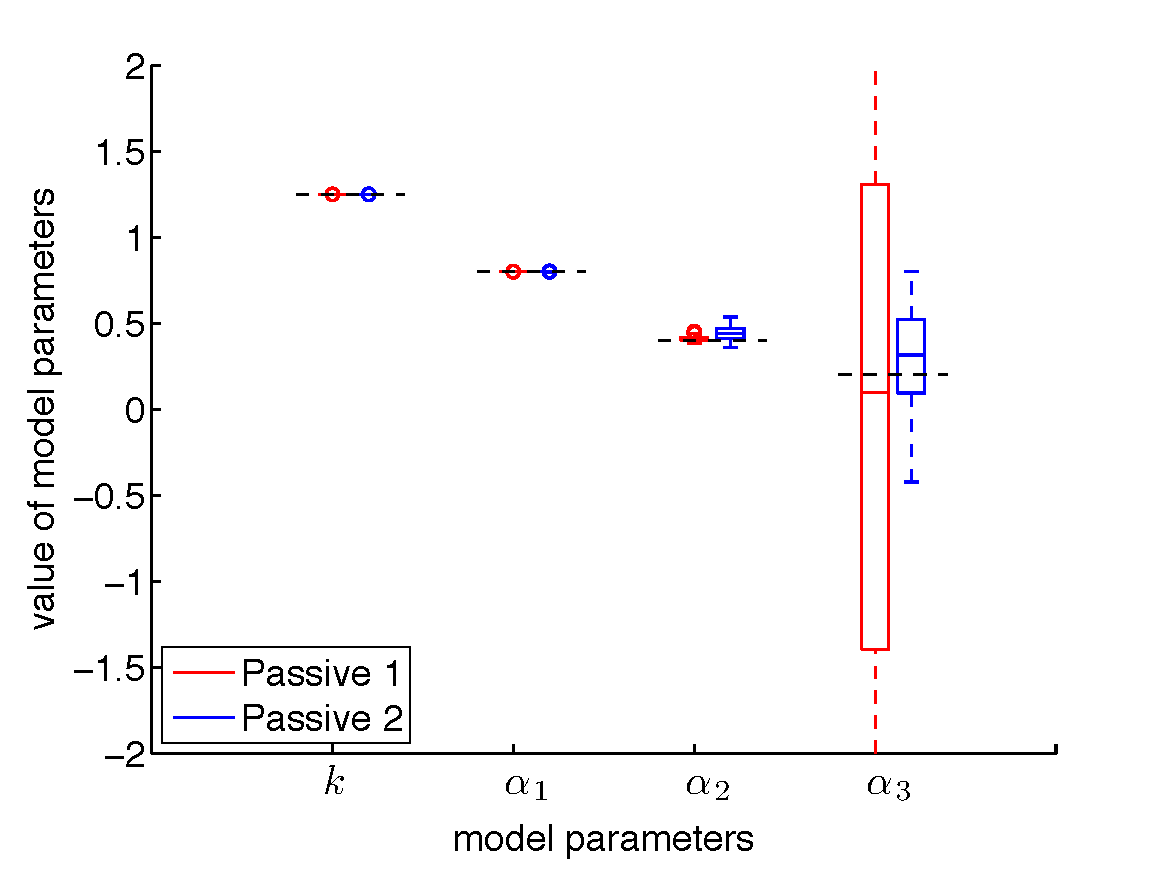
\includegraphics[width = 3 in]{ES_parameters_without_noise}
	\caption{This plots shows the distributions of the evolved models with the highest fitness in the $100000^\textrm{th}$ generation in the simple evolutions with a single population. Each box corresponds to 100 evolution runs. The dotted lines correspond to the values of the four parameters that the system is expected to learn (i.e. those of the agent). From top to bottom, these are 1.25, 0.8, 0.4, 0.2, respectively. Note that in order to zoom in on the relevant range, some boxes and outliers are omitted from the plot. \label{fig:evolution}}
\end{figure}

\begin{table}[!t] 
\caption{This table shows a comparison of all approaches. The numbers show the relative errors of the evolved parameters (median values over 100 runs) with respect to the parameters of the agent (in absolute percentage).} 
\renewcommand{\arraystretch}{1.1}
\centering % used for centering table 
\begin{tabular}{l l l l l l} % left justifying (4 columns) 
\hline\hline  %inserts double horizontal lines
 & $k$ & $\alpha_1$ & $\alpha_2$ & $\alpha_3$ &  \\  
%heading 
\hline   % inserts single horizontal line
Interactive (TL) & $0.024$ & $0$ & $0.025$ & $0.15$\\ % inserting body of the table 
Passive 1 (TL) & $1.2$ & $14.3$ & $7.8\times10^4$ & $2.3\times10^5$\\ 
Passive 2 (TL) & $0.7$ & $5.74$ & $1.3\times10^4$ & $3.3\times10^5$\\ 
Passive 1 (SPEA) & $0$ & $0$ & $1.2$ & $48.7$ \\ 
Passive 2 (SPEA) & $0$ & $0$ & $9.8$ & $48.5$ \\  % [1ex] adds vertical space 
CoEAIM & $4.0\times10^{-5}$ & $4.9\times10^{-5}$ & $1.1\times10^{-3}$ & $2.5\times10^{-4}$ \\  % [1ex] adds vertical space 
%\cline{4-5}
\hline %inserts single line 
\end{tabular} 
\label{table:relative_accuracy} % is used to refer this table in the text 
\end{table} 

In order to compare \textit{Turing Learning} against a more traditional approach, we used a simple evolution where a single population of models evolves. We call this method SPEA. As there are now no classifiers, an interactive approach is not possible, and thus we conducted $100$ evolutionary runs for the Passive 1 and Passive 2 methods of changing the light intensity in the agent's environment. The structure of the evolution is identical to the sub-algorithms used in the coevolution, except for the fitness evaluation step. Now, in each generation, $100$ experiments are performed on the agent using $100$ randomly generated intensity patterns. The $100$ intensity patterns are used to evaluate a model $100$ times. The average square error between the model's and the agent's speed sequences is used as the model's fitness. Each evolutionary run lasts $100,000$ generations. In other words, the number and duration of experiments on the agent is kept the same as that in the coevolutionary approach, as outlined in Section~\ref{sec:simulation_setup_deterministic}.

\begin{figure}[!t]
	\centering
	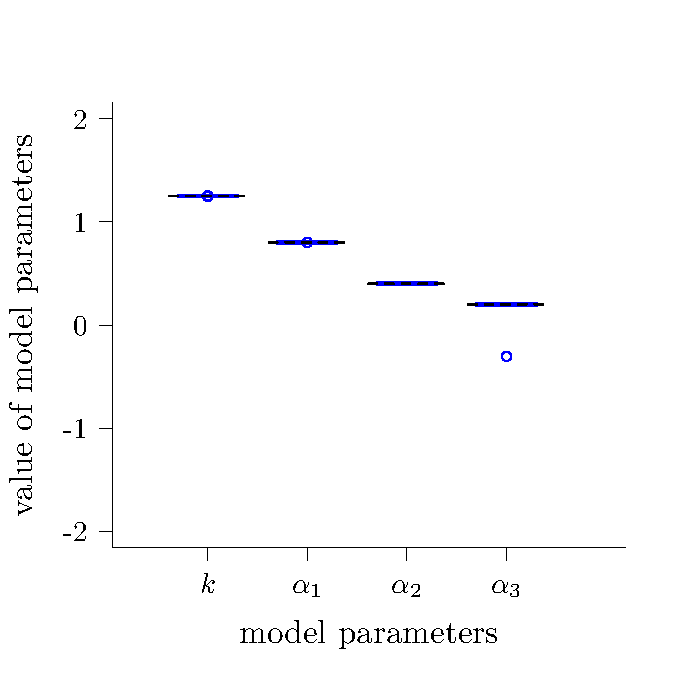
\includegraphics[width = 3 in]{model_parameters_box_CoEATM_deterministic}
	\caption{This plots shows the distributions of the evolved models with the highest fitness in the $100000^\textrm{th}$ generation in the simple evolutions with a single population. Each box corresponds to 100 coevolution runs. The dotted lines correspond to the values of the four parameters that the system is expected to learn (i.e. those of the agent). From top to bottom, these are 1.25, 0.8, 0.4, 0.2, respectively. \label{fig:model_parameters_box_CoEATM_deterministic}}
\end{figure}

Figure~\ref{fig:evolution} reveals that the evolution is able to identify parameters $k$, $\alpha_1$, $\alpha_2$, but not $\alpha_3$. Note that, apart from the single-population evolution not being able to consistently identify the parameter $\alpha_3$, they also rely on a pre-defined metric for their operation; in this case, computed as the square error between the model's and the agent's speed sequences. 

\subsubsection{Coevolution of Inputs and Models}\label{sec:coevolution_inputs_and_models_deterministic_interaction}

In this section, we compare \textit{Turing Learning} with another coevolutionary system identification method, in which inputs and models competitively coevolve. In particular, we use the classifiers to generate sequences of inputs (in this case, light intensity). The models are optimized through minimizing the square error of speed between the agent and models, given the same sequence of inputs generated by the classifiers. The classifiers compete with the models through generating inputs that cause the maximum disagreement between the model's prediction and the agent's output, which is similar to the concept in~\cite{Bongard2005_tevc}. Note that in this case the classifiers are only used for generating the inputs and they do not make judgments. We call this method CoEAIM. Figure~\ref{fig:model_parameters_box_CoEATM_deterministic} shows the results of CoEAIM. As we can see, the model parameters are also identified with a high accuracy. In other words, there is no `true' interaction between the agent and classifiers during the experiments in \textit{Turing Learning} when investigating the deterministic behavior. The classifiers only need to learn how to generate a fixed sequence of inputs to extract all the information from the agent. For a comparison of all approaches, see Table~\ref{table:relative_accuracy}. 

In order to further validate and highlight the benefit of \textit{Turing Learning}, we investigate the stochastic behaviors in the following section. 

\section{Case Study Two}\label{sec:case_study_two_stochastic_interaction}

\subsection{Stochastic Behavior}\label{sec:stochastic_behavior_interaction}

\begin{figure}[!t]
\centering
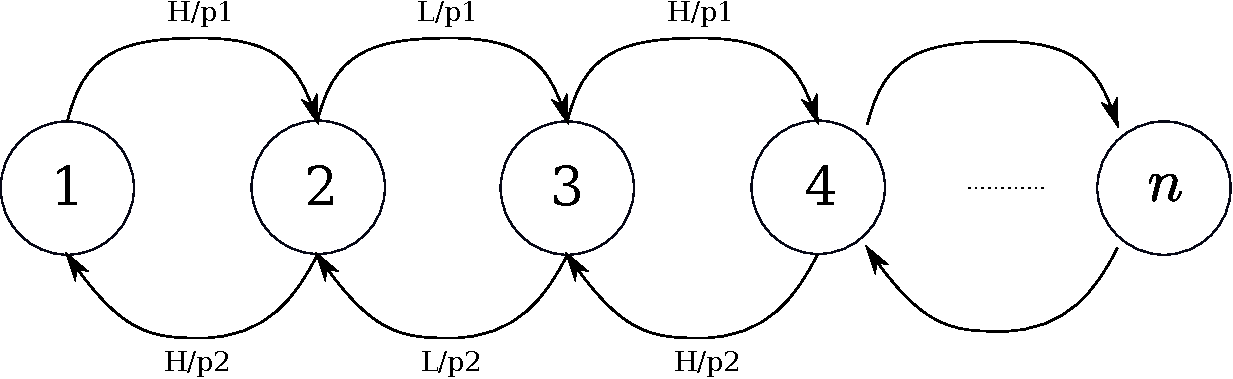
\includegraphics[width=3.5 in]{stochastic_interaction_nstates.pdf}
\caption{A state machine which represents the stochastic behavior of the agent under investigation. The initial state is 1. $p_1$, $p_2$ are probabilities. The ambient light intensity that the agent responds to has two levels: $H$ and $L$. See text for details.}
\label{fig:stochastic_behavior_n_states} 
\end{figure}

Stochastic behaviors are widely observed in the animal kingdom. Given the same stimuli, the animal may behave differently. In order to make the animal under investigation reveal all its behavioral repertoire, ethologists sometimes need to interact with the animals in real time and change the stimuli dynamically according to the animal's response. Based on this motivation, in this section we apply \textit{Turing Learning} to infer stochastic behaviors and investigate whether a machine could interact with the agent through dynamically changing the stimulus rather than generating a fixed sequence of inputs.

We will describe the stochastic behavior for the general case. It is represented as a state machine shown in Figure~\ref{fig:stochastic_behavior_n_states}. Suppose the agent has $n$ states. The agent's behavior depends on the level of the light intensity in the environment and its current state (i.e., the agent has short-term memory). For the initial state ($1$), if the light intensity is in low level ($L$), the agent keeps staying in state $1$; if the light intensity is in high level ($H$), the agent has the probability of $p_1$ to move forward to state $2$. For the middle state with even (odd) number, if the level of light intensity is $L$ ($H$), the agent has the probability of $p_1$ to move forward to another state with higher number; otherwise if the light intensity is $H$ ($L$), it has the probability of $p_2$ to move back to a previous state with lower number. When the agent is in the final state, $n$, its behavior is similar to that in the middle state. The only difference is the agent never moves forward. Figure~\subref*{fig:stochastic_interaction_2states} and Figure~\subref*{fig:stochastic_interaction_3states} show the agent behavior with 2 and 3 states, respectively. These are the two behaviors to be investigated in the thesis. 

%For the middle state, $s \in {2, 3, \cdots, n-1}$, if the level of light intensity is immediately switched (from $H$ to $L$ or from $L$ to $H$) and keeps in that level after the agent enters that state, it has the probability of $p1$ to move forward to another state with a higher number (e.g., from state $2$ to state $3$); if the light intensity is not switched, the agent would move back to a previous state with a probability of $p2$. 
\begin{figure}[!t]%htbp
	\centering
		\subfloat[2 states \label{fig:stochastic_interaction_2states}]{%
			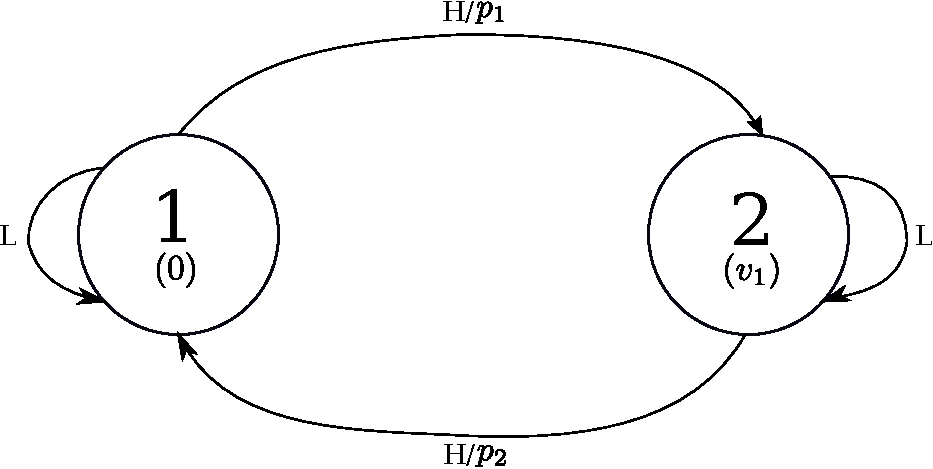
\includegraphics[width=3.0 in]{stochastic_interaction_2states.pdf}
		}\\
		\subfloat[3 states\label{fig:stochastic_interaction_3states}]{%
			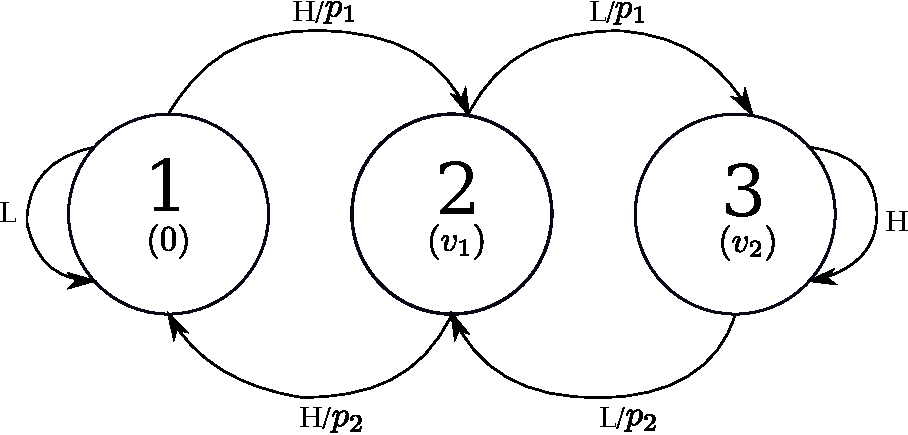
\includegraphics[width=3.0 in]{stochastic_interaction_3states.pdf}
		}
		\caption{The stochastic behaviors with (a) 2 states and (b) 3 states under invesitgation. $p_1$ and $p_2$ are probabilities. For all the other cases (e.g., $H/(1-p_1)$), the agent keeps staying in the same state.\label{fig:stochastic_interaction_case_study}}
\end{figure}

In the agent's behavior, $p_1$ is selected to a low value and $p_2$ is set to a high value. As a consequence of this choice, the agent has a low chance of moving forward to a state with a higher number and thus the higher state has lower observability. The classifiers need to learn how to interact with the agent to infer all its behavioral repertoire.

For a proof-of-concept study, we assume that the agent moves in one-dimensional space and moves at a consistent speed in each state. Suppose the agent stays static and its initial state is known. The system identification task is to identify the parameters of the agent's other states (i.e., $v_1$ and $v_2$ shown in Figure~\ref{fig:stochastic_interaction_case_study}) and the two probabilities, $p_1$ and $p_2$. The speed of the agent in each state is chosen arbitrarily. $p_1$ and $p_2$ are chosen to have a value of $0.1$ and $1.0$. This makes the agent's state with higher number has lower observability.

In order to make the agent stay in the state with higher number as long as possible, the classifiers need to capture the point when the agent starts to move forward from a state with a lower number to a state with a higher number and switches the level of light intensity immediately. This makes it easier for \textit{Turing Learning} to learn the behavior as the state can be observed for a sufficient time. If the classifiers fail to do that, the agent would immediately move to the previous state with lower number. 

For the 2-state machine shown in Figure~\subref*{fig:stochastic_interaction_2states}, $v_1$ is selected to be $0.5$; for the 3-state machine shown in Figure~\subref*{fig:stochastic_interaction_3states}, $v_1$ and $v_2$ are selected to be $0.5$ and $1.0$, respectively. Therefore, the parameters to be identified for the 2-state and 3-state agent behavior are:

\begin{equation}\label{eq:parameters_2_states}
\mathbf{q}_1 = (v, p_1, p_2) = (0.5, 0.1, 1.0).
\end{equation}

\begin{equation}\label{eq:parameters_3_states}
\mathbf{q}_2 = (v_1, v_2, p_1, p_2) = (0.5, 1.0, 0.1, 1.0).
\end{equation}

\subsection{Simulation Setup}\label{sec:simulation_setup_stochastic_interaction}

For \textit{Turing Learning}, we still used three setups: ``Interactive'', ``Passive 1'' and ``Passive 2'', as discussed in Section~\ref{sec:simulation_setup_deterministic_interaction}. We also compared \textit{Turing Learning} with the two metric-based methods (SPEA and CoEAIM) described in Section~\ref{sec:single_population_EA_deterministic_interaction} and Section~\ref{sec:coevolution_inputs_and_models_deterministic_interaction}, respectively. Note that for each setup, we added a certain amount of noise into the measurement of speed. This is realized by multiplying the agent's real speed with a random value in $[0.95, 1.05]$ in each time step. 

\subsection{Results: Two States}\label{sec:results_interaction_stochastic_2states}

In this section, we compare and analyze the results obtained using the methods discussed in the previous section (\ref{sec:simulation_setup_stochastic_interaction}) for inferring the 2-state agent behavior shown in Figure~\subref*{fig:stochastic_interaction_2states}.

\subsubsection{Analysis of Evolved Models}
\begin{figure}[!t]%htbp
	\centering
		\subfloat[Turing Learning \label{fig:parameters_box_coevolution_nometric}]{%
			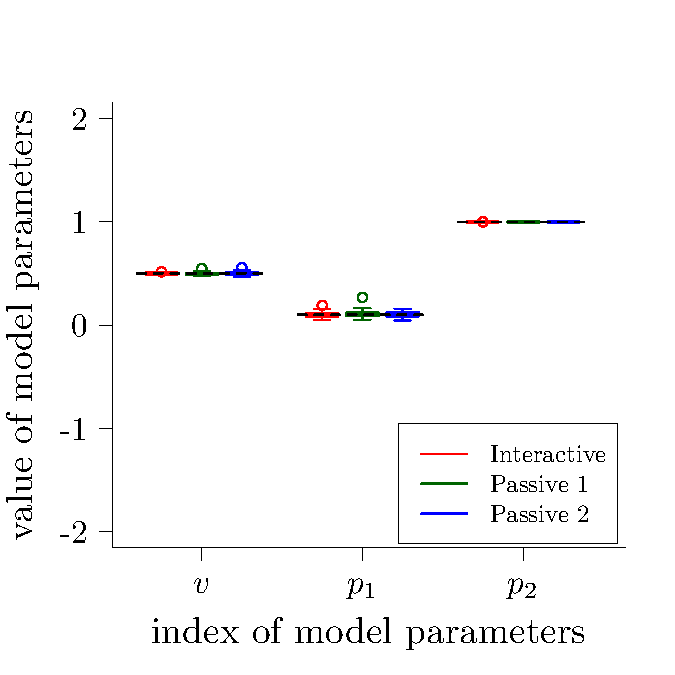
\includegraphics[width=2.8 in]{parameters_box_coevolution_nometric_2states.pdf}
		}\\
		\subfloat[SPEA \label{fig:parameters_box_coevolution_metric}]{%
			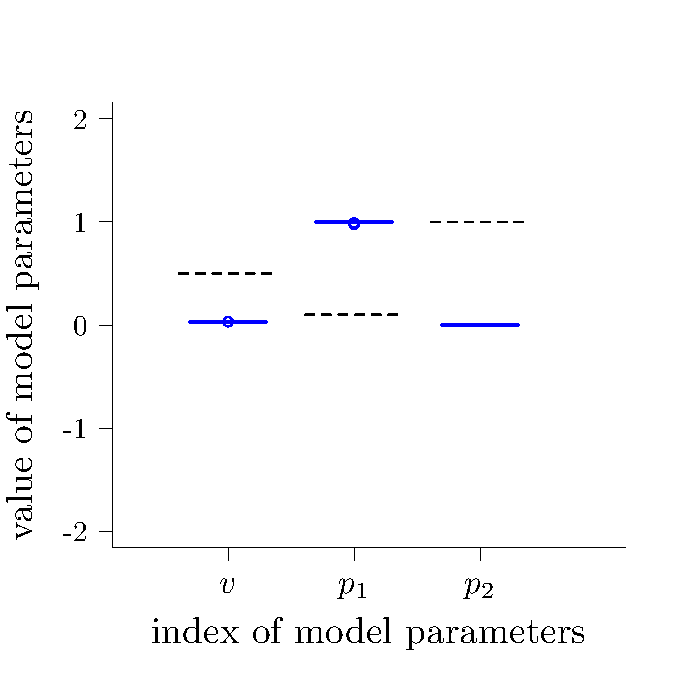
\includegraphics[width=2.8 in]{parameters_box_coevolution_metric_2states.pdf}
		}\\
		\subfloat[CoEAIM \label{fig:parameters_box_evolution_metric}]{%
			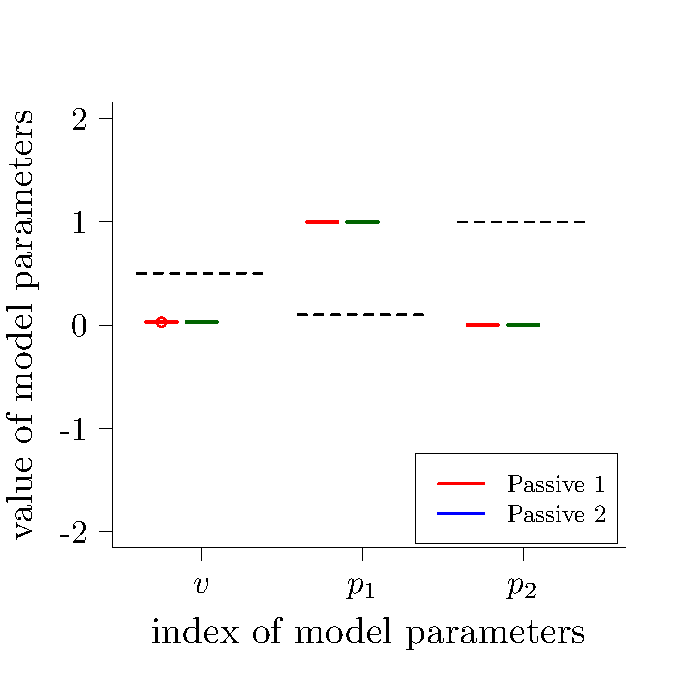
\includegraphics[width=2.8 in]{parameters_box_evolution_metric_2states.pdf}
		}
		\caption{This plot shows the distributions of the evolved models with the highest subjective fitness in the $1000^\textrm{th}$ generation in the coevolutions. Each box corresponds to $30$ coevolution runs. The dotted lines correspond to the values of the three parameters that the system is expected to learn (i.e. those of the agent). See text for details.\label{fig:parameters_box_stochastic_two states}}
\end{figure}

Figure~\ref{fig:parameters_box_stochastic_two states} shows a box plot with the parameters of the evolved models with the highest subjective fitness in the $1000^\mathrm{th}$ generation for (a) \textit{Turing Learning}, (b) SPEA, and (c) CoEAIM. Using \textit{Turing Learning}, the system identified all parameters of the agent with good accuracy. For the other two metric-based methods, all the three parameters are not learned well. Instead, the three evolved parameters converge into three different values: $v_1 \rightarrow 0.0$, $p_1 \rightarrow 1.0$, $p_2 \rightarrow 0.0$. The failure of SPEA and CoEAIM can be explained as follows. As the behavior is stochastic, given the same sequence of inputs the agent would probably exhibit different behaviors. Therefore, quantitatively measuring the difference between the models and agent (e.g., using square error) would not lead the model parameters to converge into their true values. For all methods, the means (standard deviations) of the AEs of each parameter of the evolved model with the highest fitness in the final generation over $30$ coevolution runs are shown in Table~\ref{table:relative_accuracy_stochastic_2states}. Clearly, \textit{Turing Learning} infers the stochastic behavior significantly better than the two metric-based methods. There is no significant difference among ``Interactive'', ``passive 1'' and ``passive 2'' setups of \textit{Turing Learning} in terms of AEs of the evolved parameters. 

\begin{table}[!t] 
\caption{This table shows a comparison of all approaches for learning the 2-state stochastic behavior shown in Figure~\ref{fig:stochastic_interaction_case_study}\textcolor{blue}{(a)}. The values show means of AEs (defined in Equation~\ref{eq:AE}) of each evolved model parameter with respect to that of the agent.} 
\renewcommand{\arraystretch}{1.1}
\centering % used for centering table 
\begin{tabular}{l l l l l} % left justifying (4 columns) 
\hline\hline  %inserts double horizontal lines
 & $v_1$ & $p_1$ & $p_2$ &  \\  
\hline   % inserts single horizontal line
Interactive (TL) & $0.003$ & $0.03$ & $1.6\times10^{-5}$ \\ % inserting body of the table 
Passive 1 (TL) & $0.01$ & $0.03$ & $1.0\times10^{-5}$ \\ 
Passive 2 (TL) & $0.02$ & $0.02$ & $1.0\times10^{-5}$ \\ 
Passive 1 (SPEA) & $0.47$ & $0.9$ & $1.0$ \\ 
Passive 2 (SPEA) & $0.47$ & $0.9$ & $1.0$ \\ 
CoEAIM & $0.47$ & $0.9$ & $1.0$ \\
%\cline{4-5}
\hline %inserts single line 
\end{tabular} 
\label{table:relative_accuracy_stochastic_2states} 
\end{table} 

In order to show the advantage of ``Interactive'' setup of \textit{Turing Learning}, we investigate the convergence of model parameters during the evolutionary process. Figure~\ref{fig:model_parameters_convergence_stochastic_2states} shows the convergence of the model parameters over generations for the three setups of \textit{Turing Learning}. As we can see, the evolved model parameters in the ``Interactive'' setup converge much faster than those in the two passive setups. For the ``Interactive'' setup, after about $100$ generations, all the three parameters converge into their true values. For the ``Passive 1'', all the parameters converge after about $200$ generations, while for the ``Passive 2'' it takes longer time. In terms of $v_1$, there is much smaller disturbance in the ``Interactive'' setup than that in the other two setups. 

\begin{figure}[!t]%htbp
	\centering
		\subfloat[Interactive \label{fig:model_parameters_convergence_nometric_interaction_2states}]{%
			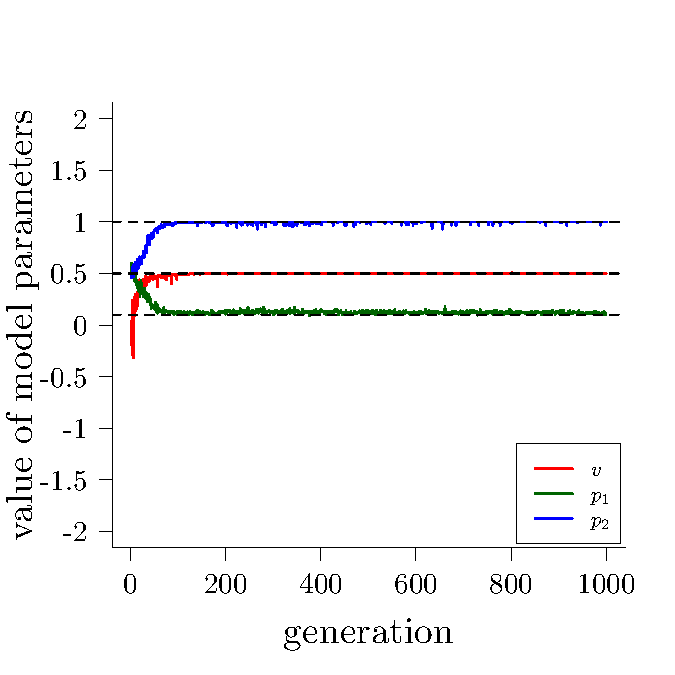
\includegraphics[width=2.8 in]{model_parameters_convergence_nometric_interaction_2states.pdf}
		}\\
		\subfloat[Passive 1 \label{fig:model_parameters_convergence_nometric_passive1_2states}]{%
			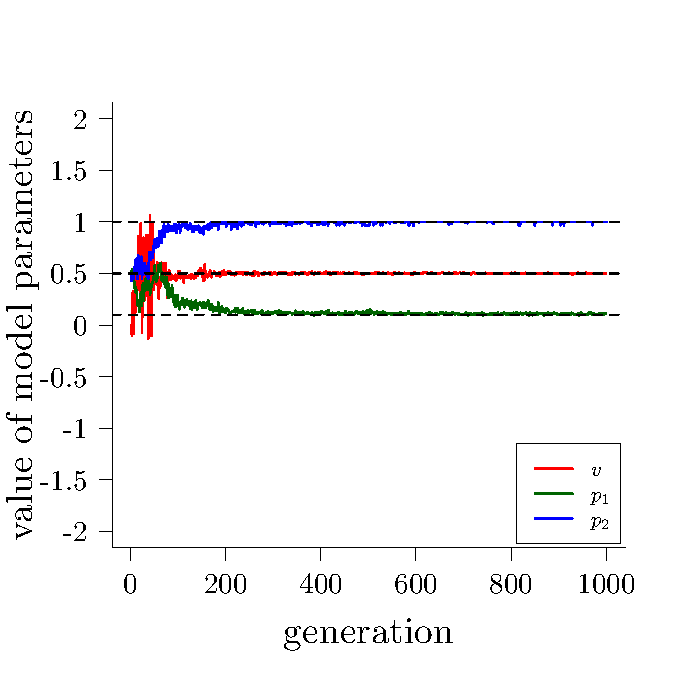
\includegraphics[width=2.8 in]{model_parameters_convergence_nometric_passive1_2states.pdf}
		}\\
		\subfloat[Passive 2 \label{fig:model_parameters_convergence_nometric_passive2_2states}]{%
			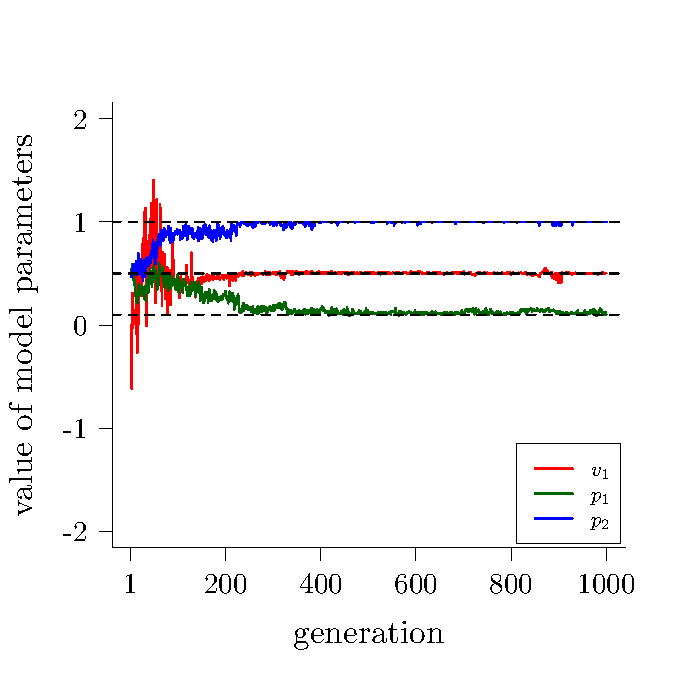
\includegraphics[width=2.8 in]{model_parameters_convergence_nometric_passive2_2states.pdf}
		}
		\caption{Evolutionary process of the evolved model parameters for (a) ``Interactive'', (b) ``Passive 1'' and (c) ``Passive 2'' setups of the metric-free method when learning the 2-state agent behavior. Curves represent mean values across 30 coevolution runs. Dotted black lines indicate true values.\label{fig:model_parameters_convergence_stochastic_2states}}
\end{figure}

\subsubsection{Analysis of Evolved Classifiers}
%
\begin{figure}[!t]
\centering
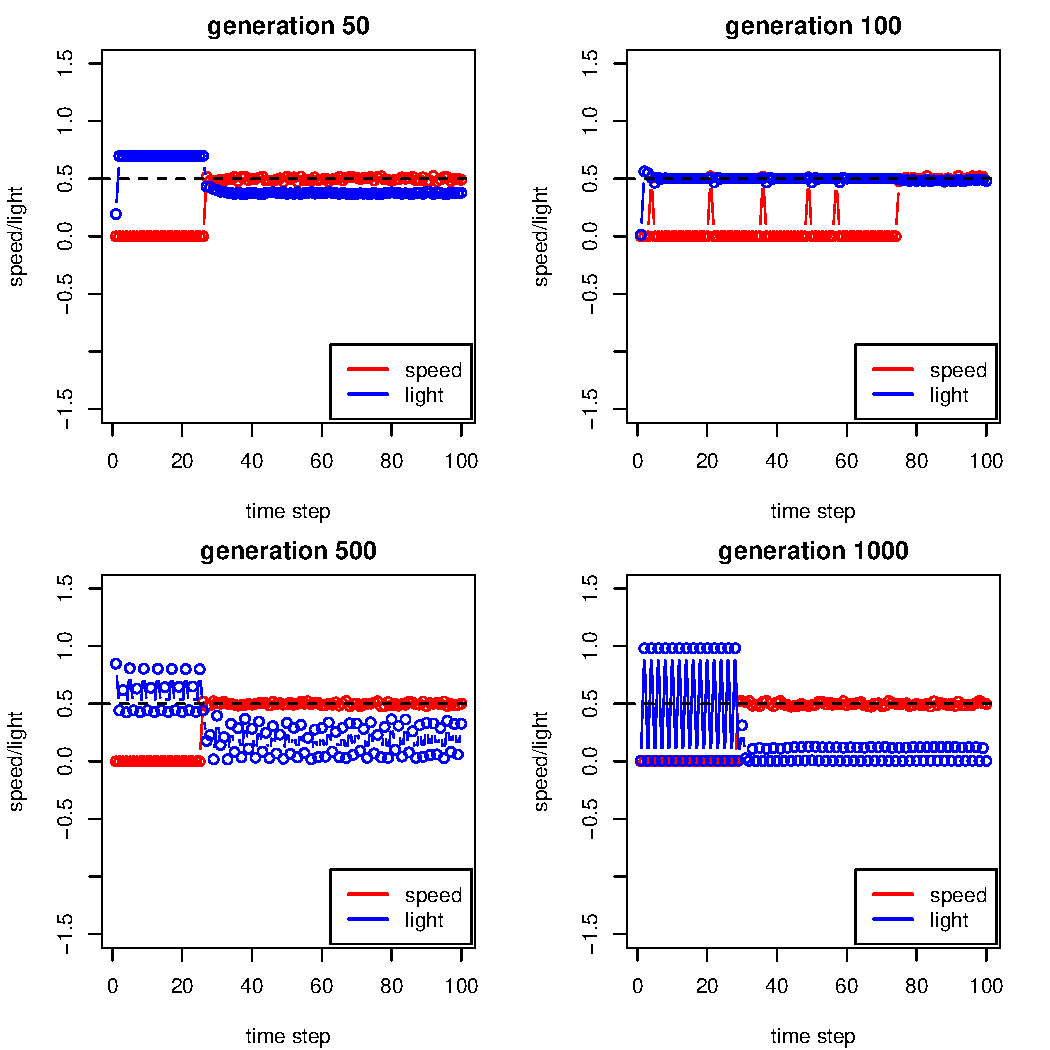
\includegraphics[width=3.5in]{classifier_interaction_2states.pdf}
\caption{This plot shows an example of how the classifier with the highest subjective fitness in different generations (of a particular coevolution run) dynamically change the light intensity to interact with the 2-state agent during a trial.}
\label{fig:classifier_interaction_2states}
\end{figure}
%
In order to investigate why the ``Interactive'' setup of \textit{Turing Learning} learns the agent behavior much faster than the two passive setups. We post-evaluated how the classifiers interact with the agent during a trial. Figure~\ref{fig:classifier_interaction_2states} shows how the classifier with the highest subjective fitness in different generations (of a particular coevolution run) interact with the agent in a trial. Similar phenomenon could be observed in other coevolution runs. 
As shown in the top left of Figure~\ref{fig:classifier_interaction_2states}, the classifier outputs $H$ level and then waits until the agent `jumps' from state $1$ to state $2$ (and this process is stochastic), and it immediately switches the light intensity from $H$ to $L$ level in order to make the agent stay in state $2$ as long as possible. Therefore, the agent's behavior in state $2$ (hidden information) can be observed longer and inferred efficiently. Note that the classifier has learned the good strategy and exhibited such `intelligent' behavior at the very beginning of the coevolution run (before $50$ generations in this case). After $500$ generations, the classifier changed the strategy a little bit. Instead of always outputting $H$ level, it keeps switching between $H$ and $L$ level until it observes the agent `jumps' from state $1$ to state $2$, and after that it immediately switches the light intensity from $H$ to $L$ level. This is unlikely to happen when generating random sequence of input.

\subsection{Results: Three States}\label{sec:results_interaction_stochastic_3states}

In order to further demonstrate the advantage of ``Interactive'' setup of \textit{Turing Learning}, this section discusses the results of inferring the 3-state stochastic agent behavior shown in Figure~\subref*{fig:stochastic_interaction_3states}. 

\subsubsection{Analysis of Evolved Models}
\begin{figure}[!t]%htbp
	\centering
		\subfloat[Turing Learning \label{fig:parameters_box_coevolution_nometric}]{%
			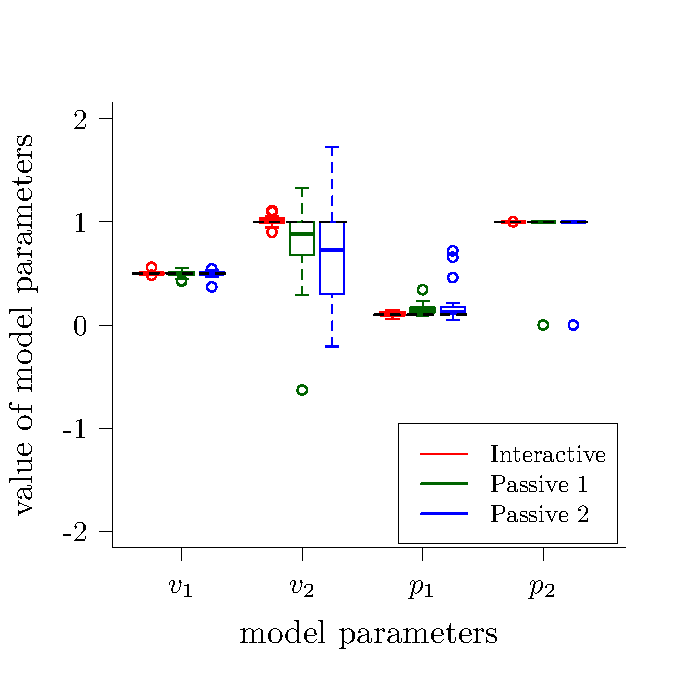
\includegraphics[width=2.8 in]{parameters_box_coevolution_nometric_3states.pdf}
		}\\
		\subfloat[SPEA \label{fig:parameters_box_coevolution_metric}]{%
			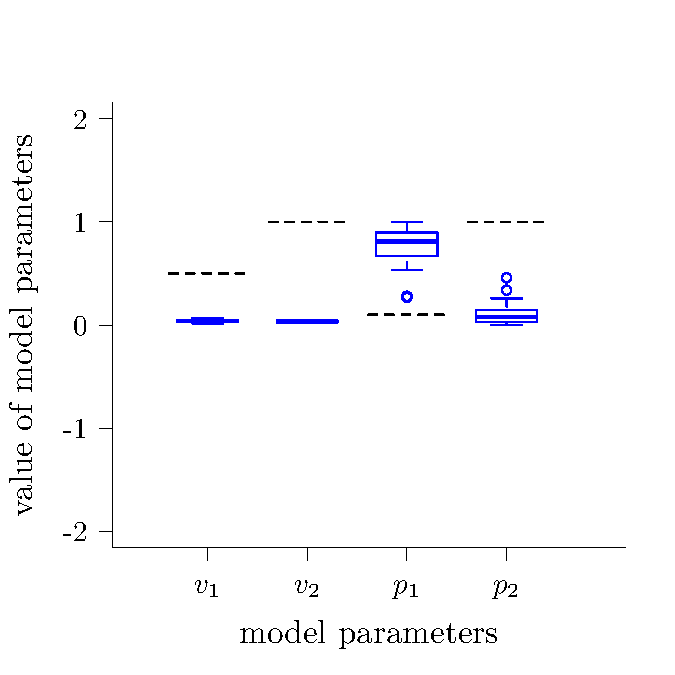
\includegraphics[width=2.8 in]{parameters_box_coevolution_metric_3states.pdf}
		}\\
		\subfloat[CoEAIM \label{fig:parameters_box_evolution_metric}]{%
			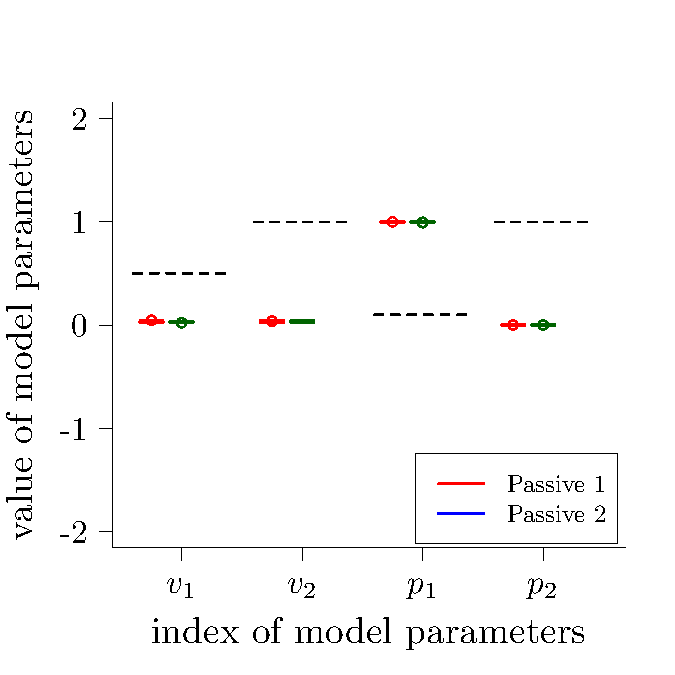
\includegraphics[width=2.8 in]{parameters_box_evolution_metric_3states.pdf}
		}
		\caption{This plot shows the distributions of the evolved models with the highest subjective fitness in the $1000^\textrm{th}$ generation in the coevolutions. Each box corresponds to $30$ coevolution runs. The dotted lines correspond to the values of the four parameters that the system is expected to learn (i.e. those of the agent). See text for details.\label{fig:parameters_box_stochastic_three_states}}
\end{figure}

Figure~\ref{fig:parameters_box_stochastic_three_states} shows the distribution of the evolved models in the $1000^\mathrm{th}$ generation for all setups. The ``Interactive'' setup of \textit{Turing Learning} is the only one that infers all the parameters of the agent with good accuracy. For the two setups using pre-defined metrics (SPEA and CoEAIM), all the parameters are not learned well. Table~\ref{table:relative_accuracy_stochastic_3states} compares the accuracy of each parameter of the evolved model with the highest fitness in the final generation over $30$ coevolution runs using all approaches.

\begin{table}[!t] 
\caption{This table shows a comparison of all approaches for inferring the 3-state agent behavior shown in Figure~\ref{fig:stochastic_interaction_case_study}\textcolor{blue}{(b)}. The values show means of AEs (defined in Equation~\ref{eq:AE}) of each evolved model parameter with respect to that of the agent.} 
\renewcommand{\arraystretch}{1.1}
\centering % used for centering table 
\begin{tabular}{l l l l l l} % left justifying (4 columns) 
\hline\hline  %inserts double horizontal lines
 & $v$ & $v_2$ & $p_1$ & $p_2$ &  \\  
\hline   % inserts single horizontal line
Interactive (TL) & $0.005$ & $0.03$ & $0.02$ & $2.0\times10^{-6}$ \\ % inserting body of the table 
Passive 1 (TL) & $0.02$ & $0.23$ & $0.05$ & $0.03$\\ 
Passive 2 (TL) & $0.02$ & $0.47$ & $0.08$ & $0.13$\\ 
Passive 1 (SPEA) & $0.47$ & $0.97$ & $0.9$ & $1.0$\\ 
Passive 2 (SPEA) & $0.47$ & $0.98$ & $0.9$ & $1.0$\\ 
CoEAIM & $0.46$ & $0.96$ & $0.67$ & $0.89$\\
%\cline{4-5}
\hline %inserts single line 
\end{tabular} 
\label{table:relative_accuracy_stochastic_3states} 
\end{table} 

Figure~\ref{fig:model_parameters_convergence_stochastic_3states} shows the evolutionary process of the models for the three setups of \textit{Turing Learning}. As we can see, all the model parameters in the``Interactive'' setup converged to their true value smoothly within about $200$ generations. For the two passive setups, $v_1$, $p_1$ and $p_2$ are learned well, but they still take longer time to converge to their true values than those of the ``Interactive'' setup. There is dramatic disturbance during the evolutionary process of $v_2$ for the passive setups, and this parameter is not learned well.

\begin{figure}[!t]%htbp
	\centering
		\subfloat[Interactive \label{fig:model_parameters_convergence_nometric_interaction_3states}]{%
			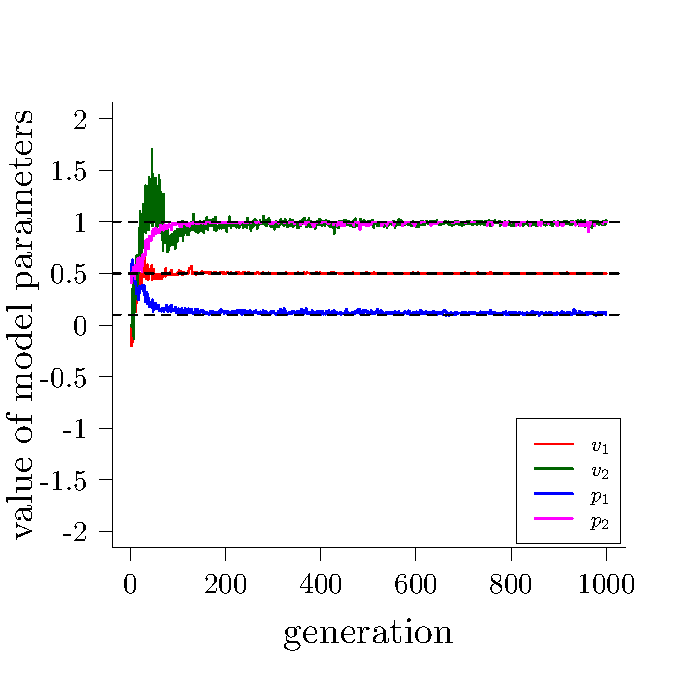
\includegraphics[width=2.8 in]{model_parameters_convergence_nometric_interaction_3states.pdf}
		}\\
		\subfloat[Passive 1 \label{fig:model_parameters_convergence_nometric_passive1_3states}]{%
			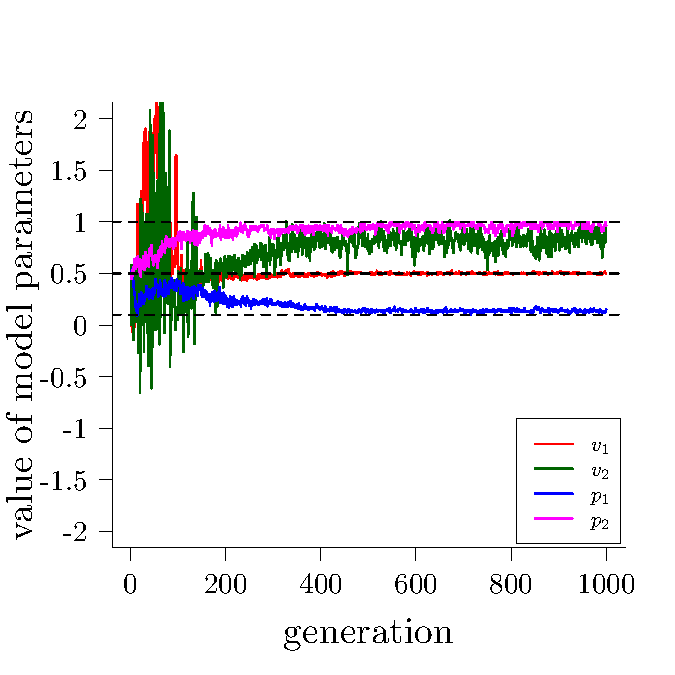
\includegraphics[width=2.8 in]{model_parameters_convergence_nometric_passive1_3states.pdf}
		}\\
		\subfloat[Passive 2 \label{fig:model_parameters_convergence_nometric_passive2_3states}]{%
			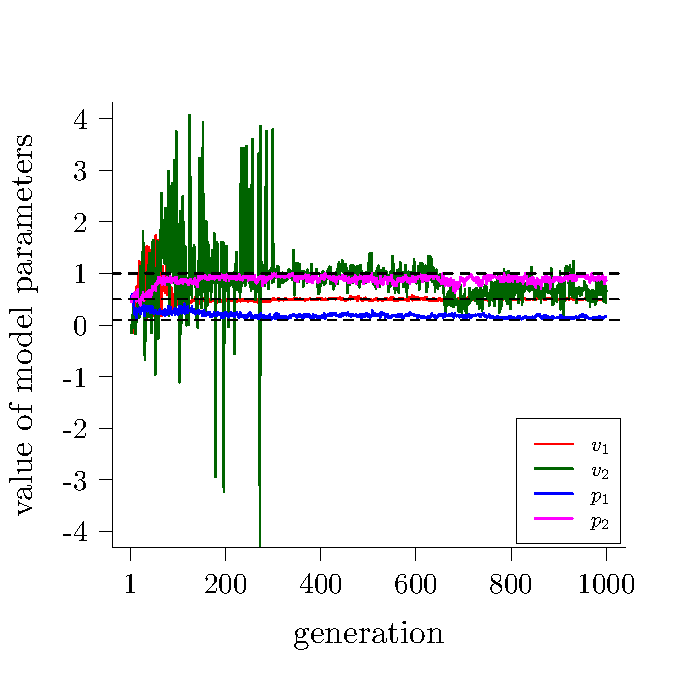
\includegraphics[width=2.8 in]{model_parameters_convergence_nometric_passive2_3states.pdf}
		}
		\caption{Evolutionary process of the evolved model parameters for (a) ``Interactive'', (b) ``Passive 1'' and (c) ``Passive 2'' setups of the metric-free method when learning the 3-state agent behavior. Curves represent mean values across 30 coevolution runs. Dotted black lines indicate true values.\label{fig:model_parameters_convergence_stochastic_3states}}
\end{figure}

\subsubsection{Analysis of Evolved Classifiers}
%
\begin{figure}[!t]
\centering
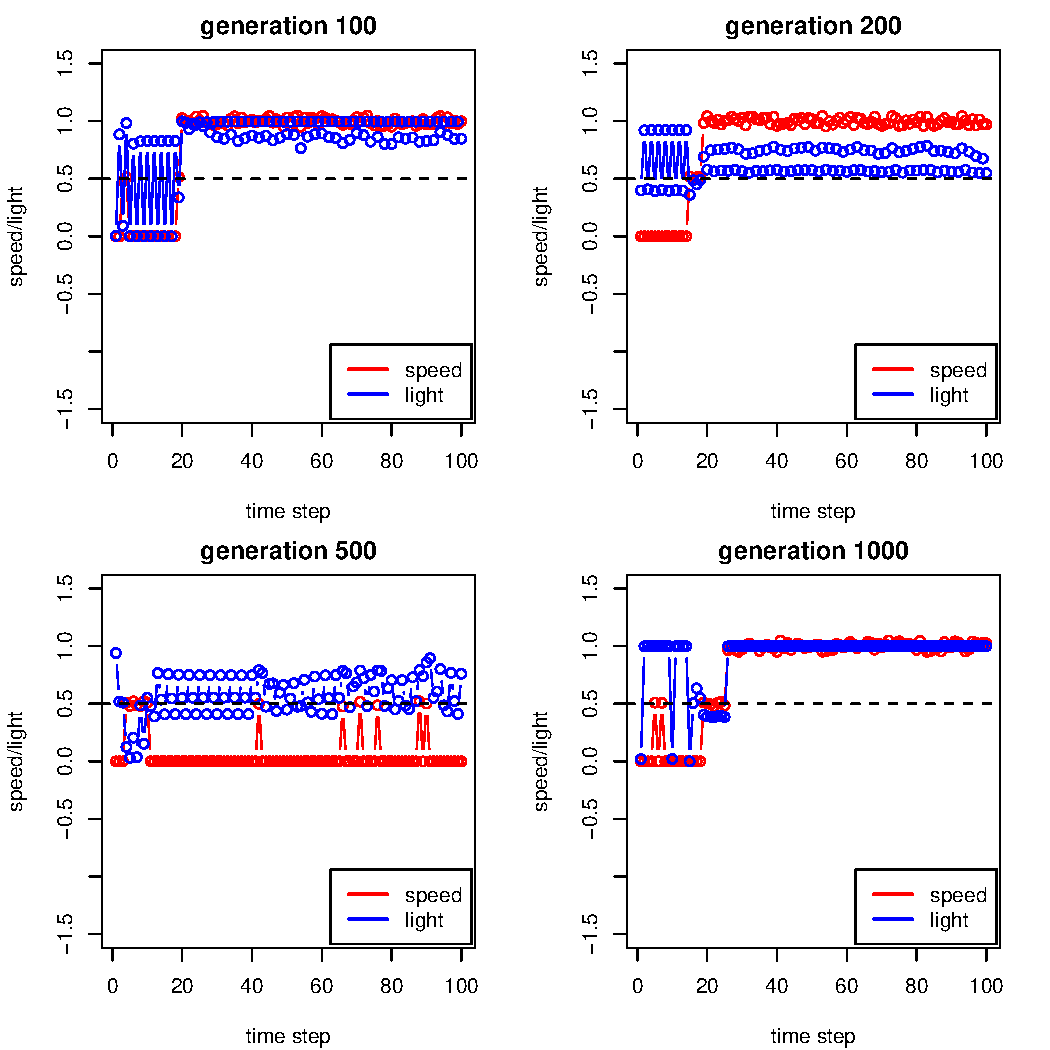
\includegraphics[width=3.5in]{classifier_interaction_3states.pdf}
\caption{This plot shows an example of how the classifier with the highest subjective fitness in different generations (of a particular coevolution run) dynamically change the light intensity to interact with the 3-state agent during a trial.}
\label{fig:classifier_interaction_3states}
\end{figure}
%

Figure~\ref{fig:classifier_interaction_3states} shows an example of how the classifier with the highest subjective fitness in different generations (of a particular coevolution run) evolved to interact with the agent. In other coevolution runs, we still observed similar phenomenon. As shown in Figure~\ref{fig:classifier_interaction_3states}, the strategy learned by the classifiers shown in $3$ of the $4$ sub-figures (corresponding to $100^\mathrm{th}$, $200^\mathrm{th}$, $1000^\mathrm{th}$ generation) is as follows. The classifier outputs $H$ first, and once the agent moves forward from state $1$ to state $2$, the classifier switches the light intensity into level $L$ and keeps it in that level. As long as the agent moves forward from state $2$ to state $3$, the classifier switches the light intensity from $L$ to $H$ and keeps the light intensity in that level. Note that the `best' classifier sometimes lost its ability to interact with the agent in the $500^\mathrm{th}$ generation shown in bottom left of Figure~\ref{fig:classifier_interaction_3states}. However, this does not influence the learning process, as long as there are still some other classifiers in the population obtain this interactive ability. 

\section{Summary}\label{sec:summary_interaction}

%This chapter has presented a new coevolutionary method that can autonomously learn the behavior of an agent, or any other agent. We have shown that, by allowing classifiers to control the stimuli in the agent's environment, the system is able to correctly identify the parameters of a relatively complex behavior. The behavior of the agent involves memory and consists of five cases where the agent's response to the stimuli is either proportional, constant or it decays exponentially over time. When only allowing the classifiers to passively observe the agent, the system was unable to fully learn its behavior. Moreover, evolutions that attempted to evolve the behavior using a simple pre-determined comparison metric could not evolve all the parameters. 

In this chapter, we extend \textit{Turing Learning} with interactive ability to autonomously learn the behavior of an agent. We have shown that, by allowing classifiers to control the stimulus in the agent's environment, the system is able to correctly identify the parameters of relatively complex behaviors. The advantage of \textit{Turing Learning} with interaction is validated using two case studies: stochastic and deterministic behaviors of an agent. In both case studies, the results show that learning through interaction can infer the agent behaviors better or faster than only through passive observation. 

When inferring the deterministic behavior, the classifiers have learned to generate a complex sequence of inputs to extract all the hidden information from the agent, which facilitates the learning process. However, generating such sequences in random is unlikely. This makes the SPEA (in which the inputs are generated randomly) fail to infer all the parameters of the agent. However, by coevolving inputs and models (CoEAIM), the system still obtained very good model accuracy in terms of all parameters. 

When inferring the stochastic behavior, the advantage of \textit{Turing Learning} with interaction is highlighted. 
It performs significantly better than the two metric-based methods (SPEA and CoEAIM) in inferring stochastic behaviors. In the ``Interactive'' setup of \textit{Turing Learning}, the classifiers learned to dynamically interact with the agent, which leading to infer all the agent's parameters in a very efficient way. The results suggest that a machine could also exhibit such intelligent behavior as observed in human behavior, and this could pave the way to further development of machine intelligence. 

%In the deterministic behavior, the post-evaluation over 100 runs through performing a grid search shows that the overall best classifier can distinguish between the agent and potential models very well, even if the latter differs only slightly in one of its parameters from the agent. The metric-free method can still perform well when the system is subjective to noise, which shows the robustness of our method. 

%Our approach does not rely on any pre-defined metric to gauge the difference of the agent and the models. Rather, such metrics are implicitly defined by the classifiers themselves, and hence incorporated into the evolutionary process. This avoids the need for metrics, which could bias the performance of a system for any specific tasks. Therefore, the feature of not relying on any pre-defined metric makes our approach task-independent and simpler to be applied to other platforms.

%The agent behavior considered here served as a case study to illustrate the proposed method. It was assumed that the models and the agent share the same structure. This facilitated the post-analysis of both the models and the classifiers that were obtained. Ethologists have often a model structure of the agent in mind~\citep{Camazine2003} and using our approach, they could identify the parameters of such a model. This could significantly reduce the number of experiments performed on the agent when compared with an approach in which the model is to be built from scratch. 
%Moreover,  and facilitates the interpretation of the results. 
%Nevertheless, our method is generic in the sense that it can, in principle, evolve the model structure as well. This is possible as the classifiers merely interact with the models and agents. They do not have prior knowledge about their structure.

%In the future, we intend to perform experiments using robots and real agents. Moreover, we will study the ability of the interactive approach to identify social interactions in groups or swarms of agents.

%It investigates in detail the effect of noise on the algorithm's behavior, under the right circumstances, noise can improve the evolutionary process by helping to maintain diversity within the populations. Moreover, it presents strategies to reduce both the number and the duration of experiments that need to be performed on the agent, without a significant degradation to the quality of the evolved models.

